%!TEX program = xelatex

\documentclass[UTF8]{ctexart}
\usepackage{ctex}

\CTEXsetup[format={\Large\bfseries}]{section}

\usepackage[version=3]{mhchem} % Package for chemical equation typesetting
\usepackage{siunitx} % Provides the \SI{}{} and \si{} command for typesetting SI units
\usepackage{graphicx} % Required for the inclusion of images
\graphicspath{{assets/}}
\usepackage{natbib} % Required to change bibliography style to APA
\usepackage{amsmath} % Required for some math elements 
\usepackage{amssymb}
\usepackage[hidelinks]{hyperref}
\usepackage{makecell} % 3 Packages for flexible tabular
\usepackage{multirow}
\usepackage{multicol}

\usepackage{pdfpages}  % include pdf pages for original data etc.

\usepackage{geometry}% 版面大小
\geometry{a4paper,scale=0.7}

\usepackage{fontspec}

\setCJKfamilyfont{hwxk}{STXingkai}% 字体
\newcommand{\hwxk}{\CJKfamily{hwxk}}

\usepackage{fancyhdr}% 页眉页脚
\fancypagestyle{EE_Digital1Exp_template}{
    \fancyhead[L]{\Large {\hwxk 南京大学电子科学与工程学院}}
    \fancyhead[R]{数字系统1实验报告}
    \fancyfoot[c]{- \thepage \ -}
    \renewcommand\footrulewidth{0pt}
}

% 4级目录
\setcounter{secnumdepth}{4}
\setcounter{tocdepth}{4}

\usepackage{graphicx} % Packages for figures
\usepackage{caption2}
\usepackage{subfigure}
\usepackage{float}

\usepackage{listings} % Packages for code block
\usepackage{xcolor}

% for verilog code coloring
\definecolor{vgreen}{RGB}{104,180,104}
\definecolor{vblue}{RGB}{49,49,255}
\definecolor{vorange}{RGB}{255,143,102}

\lstdefinestyle{verilog-style}
{
    language=Verilog,
    basicstyle=\small\ttfamily,
    keywordstyle=\color{vblue},
    identifierstyle=\color{black},
    commentstyle=\color{vgreen},
    numbers=left,
    numberstyle=\tiny\color{black},
    numbersep=10pt,
    tabsize=8,
    moredelim=*[s][\colorIndex]{[}{]},
    literate=*{:}{:}1
}

\makeatletter
\newcommand*\@lbracket{[}
\newcommand*\@rbracket{]}
\newcommand*\@colon{:}
\newcommand*\colorIndex{%
    \edef\@temp{\the\lst@token}%
    \ifx\@temp\@lbracket \color{black}%
    \else\ifx\@temp\@rbracket \color{black}%
    \else\ifx\@temp\@colon \color{black}%
    \else \color{vorange}%
    \fi\fi\fi
}
\makeatother

\usepackage{trace}




%设置图片、表格编号
\renewcommand{\thetable}{\thesubsection{}-\arabic{table}}
\renewcommand{\thefigure}{\thesubsection{}-\arabic{figure}}
\renewcommand{\thefigure}{\thesubsection{}-\arabic{equation}}
\usepackage{amsmath}
\numberwithin{figure}{subsection}
\numberwithin{table}{subsection}
\numberwithin{equation}{subsection}

\setlength\parindent{6pt} % Removes all indentation from paragraphs

\renewcommand{\labelenumi}{\alph{enumi}.} % Make numbering in the enumerate environment by letter rather than number (e.g. section 6)

%\usepackage{times} % Uncomment to use the Times New Roman font

%----------------------------------------------------------------------------------------
%	DOCUMENT INFORMATION
%----------------------------------------------------------------------------------------

\title{\textbf{实验四\ 计数器:硬件电路}} % Title

\author{电子科学与工程学院\ 刘时宜\ 201180078} % Author name

\date{} % Date for the report

\begin{document}

\pagestyle{EE_Digital1Exp_template}

\maketitle % Insert the title, author and date

\begin{center}
    \begin{tabular}{l r}
    实验日期: & 2021年12月07日 \\ % Date the experiment was performed
    指导老师: & 高健 % Instructor/supervisor
    \end{tabular}
    \par 点击目录、书签栏、以及行文中的图表标号的均可跳转至相应页面
    \end{center}
    
% If you wish to include an abstract, uncomment the lines below
% \begin{abstract}
% Abstract text
% \end{abstract}

\tableofcontents

\section{实验目的}
\begin{enumerate}
    \item 利用计数器芯片与数码管搭建计数器硬件电路
\end{enumerate}

\section{实验仪器与主要器材}
\begin{center}
    \begin{tabular}{ll}
        \textbf{仪器:} & \\
        Basys3 FPGA 开发板 & 1台\\
        KEYSIGHT DSOX1102AG 示波器 & 1台\\
        示波器高频探头 & 1套\\
        ROGOL DM3068 万用表 & 1台\\
        \textbf{软件:} & \\
        Multisim & 14.1 \\
        \textbf{芯片:} & \\
        74LS90 & 1片 \\
        74LS47 & 1片 \\
        \textbf{耗材:} & \\
        导线 & 若干 \\
    \end{tabular}
\end{center}

\section{实验原理}
\par 计数器在数字系统中广泛使用,可以用于对时钟脉冲计数、分频、定时、进行数学运算等。
\par 计数器种类繁多。如果按照计数器中的触发器是否同时翻转分类,可以将计数器分为同步式和异步式两种。同步计数器中,当时钟脉冲输入时触发器的翻转同时发生,而在异步计数器中,触发器的翻转又先后,不是同时发生的。
\par 如果按照计数过程中数字的增减分类,可以分为加法计数器、减法计数器以及可逆计数器。随着计数脉冲的不断输入而作递增的计数器称为加法计数器,作递减计数的称为减法计数器,可增可减的称为可逆计数器。
\par 本实验中用到的计数器为异步加法计数器。将其接到BCD译码器及数码管,即可获得计数显示。

\section{实验过程}
\subsection{十进制计数器}
\subsubsection{原理电路}
\par 实验电路原理图如\ref{10 theory cir}所示。其中将74LS90的QA端接回INB触发端口,利用74LS90芯片特性构成十进制计数器。74LS90产生加法计数的BCD码后将其送至74LS47BCD显示译码器,进行译码并将输出送至数码管进行显示输出。

\begin{figure}[H]
    \begin{center}
        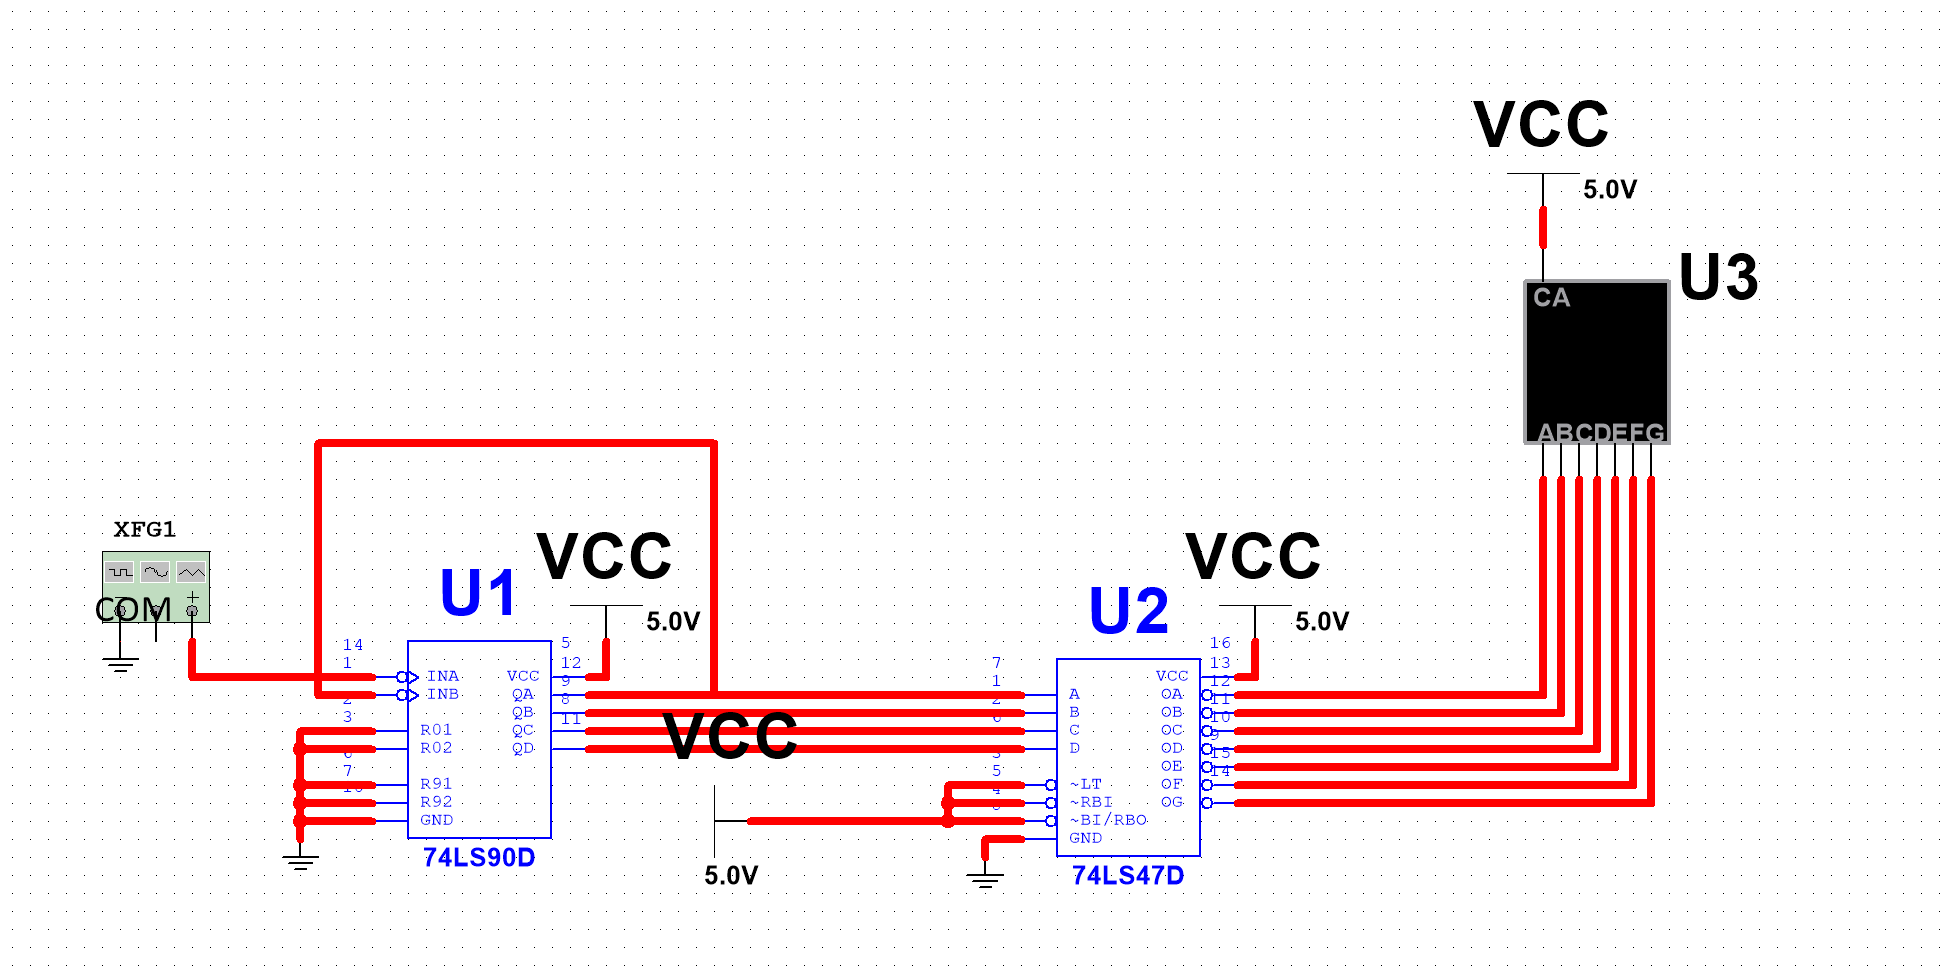
\includegraphics[width=0.8\textwidth]{design/10 circuit.png}
    \end{center}
    \caption{十进制计数器:原理电路}
    \label{10 theory cir}
\end{figure}

\subsubsection{电路实验}
\par 依据原理图,搭建硬件电路如图\ref{10 cir}所示。输入信号INA接信号发生器方波。方波参数为高电平\SI{5}{\volt},低电平\SI{0}{\volt},频率\SI{3}{\hertz}。

\begin{figure}[H]
    \begin{center}
        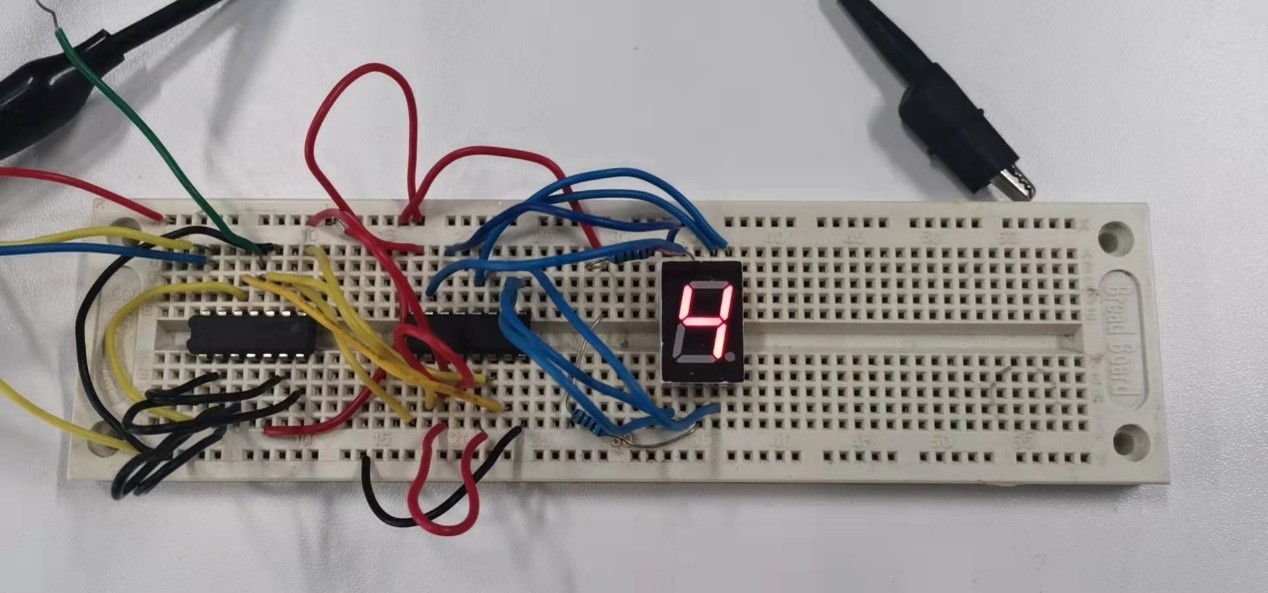
\includegraphics[width=0.8\textwidth]{10/circuit.jpg}
    \end{center}
    \caption{十进制计数器:硬件电路}
    \label{10 cir}
\end{figure}

\par 打开电源、打开信号源,观察实验现象。\SI{3}{\hertz}时电路现象已录制为"十进制计数器.mp4",附在邮件插件中。
\par 加大信号源频率,使用示波器观察计数器各引脚输出。其中信道1为时钟信号,信道2分别为各位输出。实验结果如图\ref{10 osci}所示。

\begin{figure}[H]
    \centering
    \subfigure[QA]{
    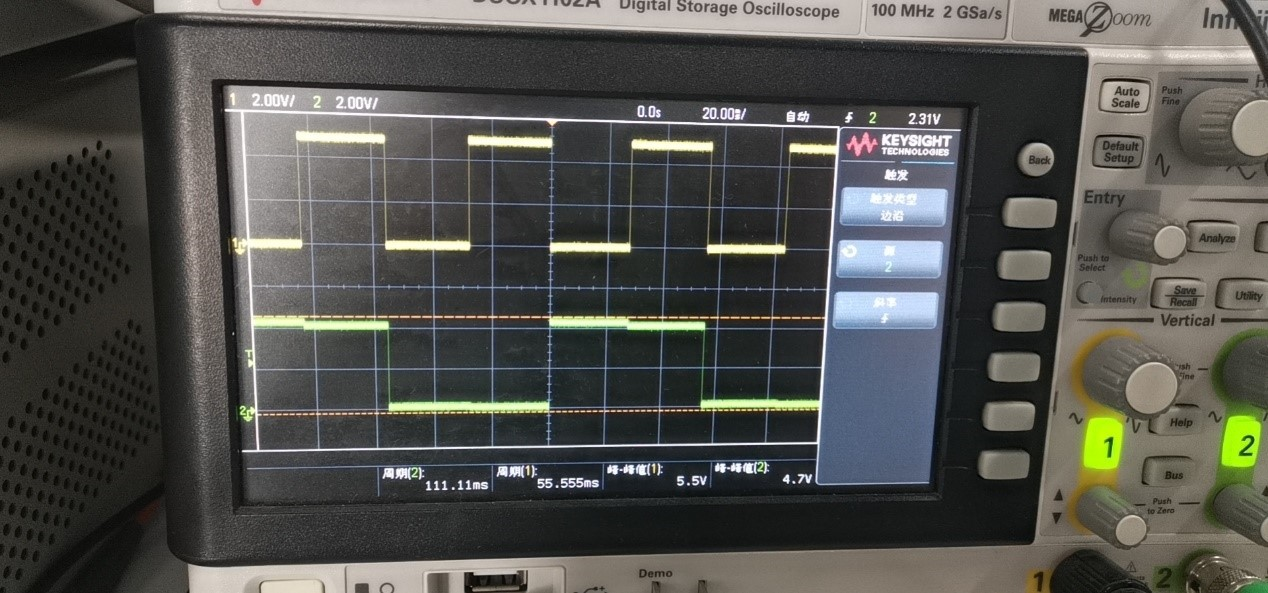
\includegraphics[width=0.45\textwidth]{10/QA.jpg}}
    \subfigure[QB]{
    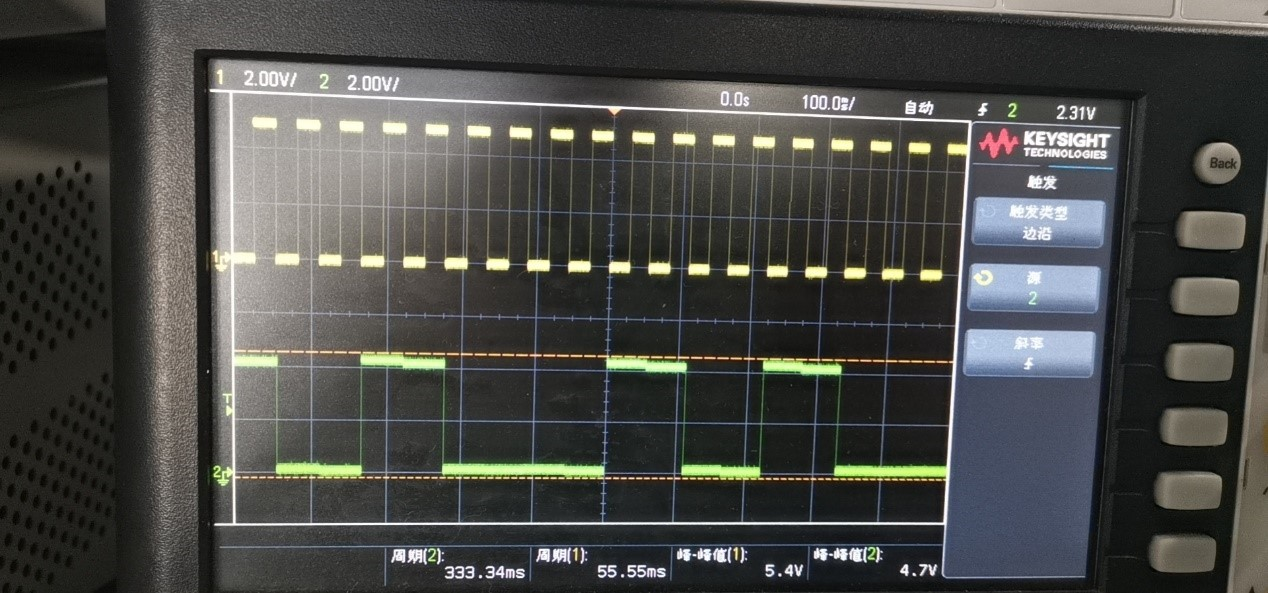
\includegraphics[width=0.45\textwidth]{10/QB.jpg}}
    \subfigure[QC]{
    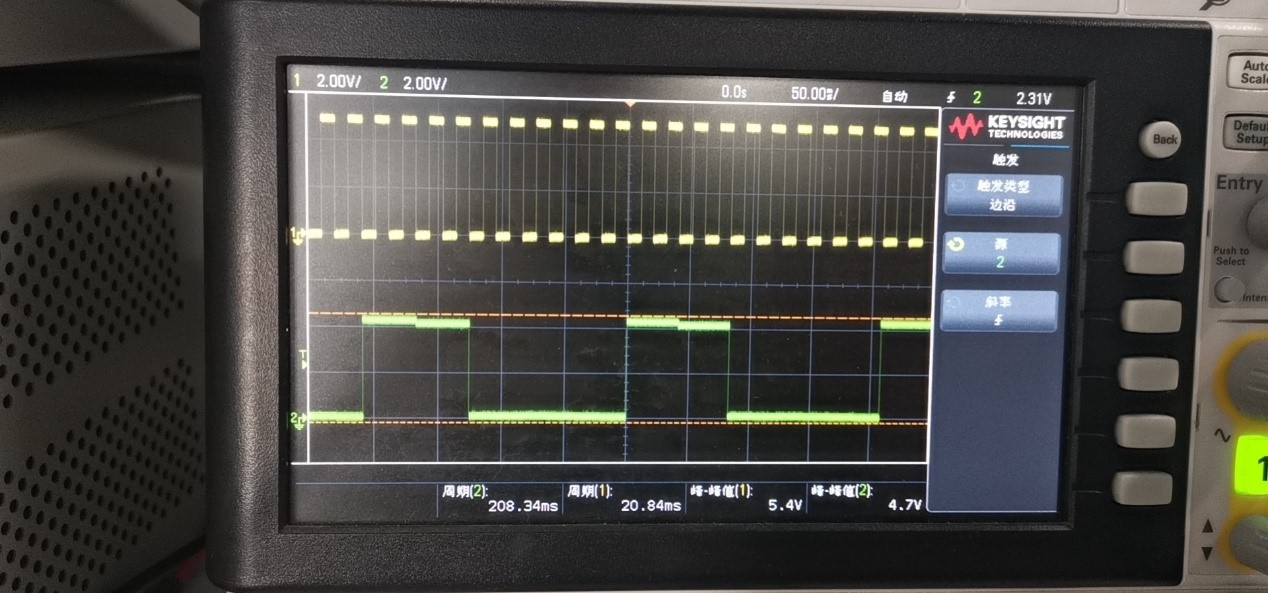
\includegraphics[width=0.45\textwidth]{10/QC.jpg}}
    \subfigure[QD]{
    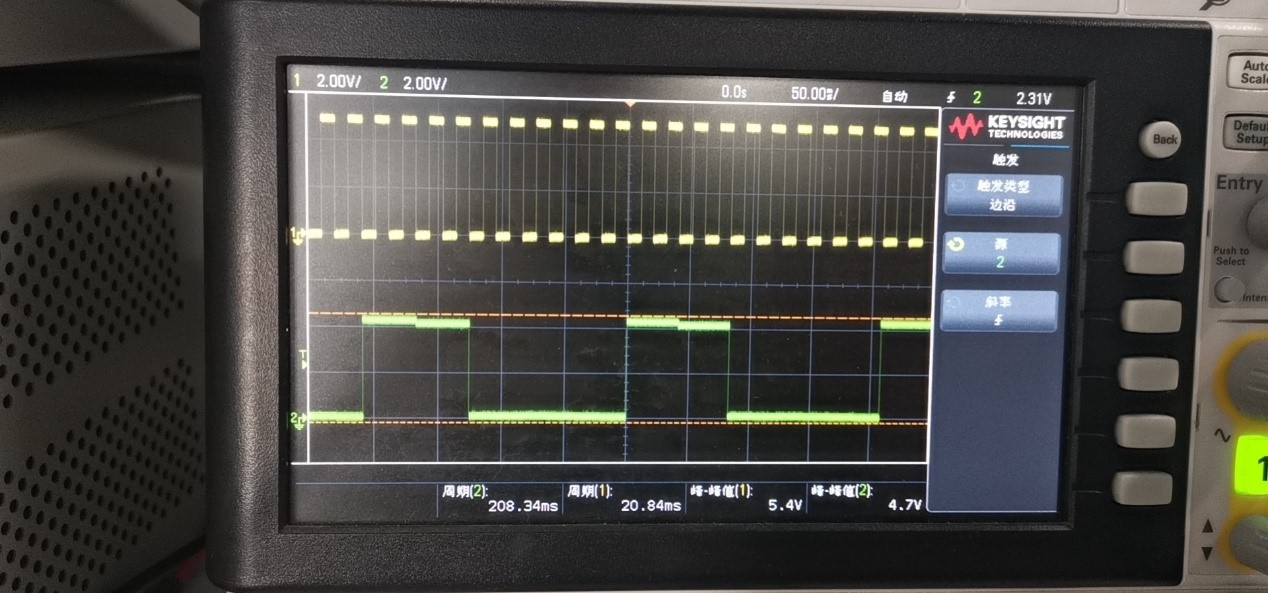
\includegraphics[width=0.45\textwidth]{10/QD.jpg}}
    \caption{十进制计数器:引脚波形}
    \label{10 osci}
\end{figure}

\par 可以看到,电路现象与各引脚波形与理论相符,成功搭建了十进制计数器硬件电路。


\subsection{六进制计数器:置零法}
\subsubsection{原理电路}
\par 实验电路原理图如\ref{6-0 theory cir}所示。在十进制计数器的基础上,将QB、QC引回电路置零端,使得电路输出二进制6,即“0110”时,计数器归零。由此使计数器输出在0、1、2、3、4、5,共计6个稳态间跳变,实现六进制计数器。

\begin{figure}[H]
    \begin{center}
        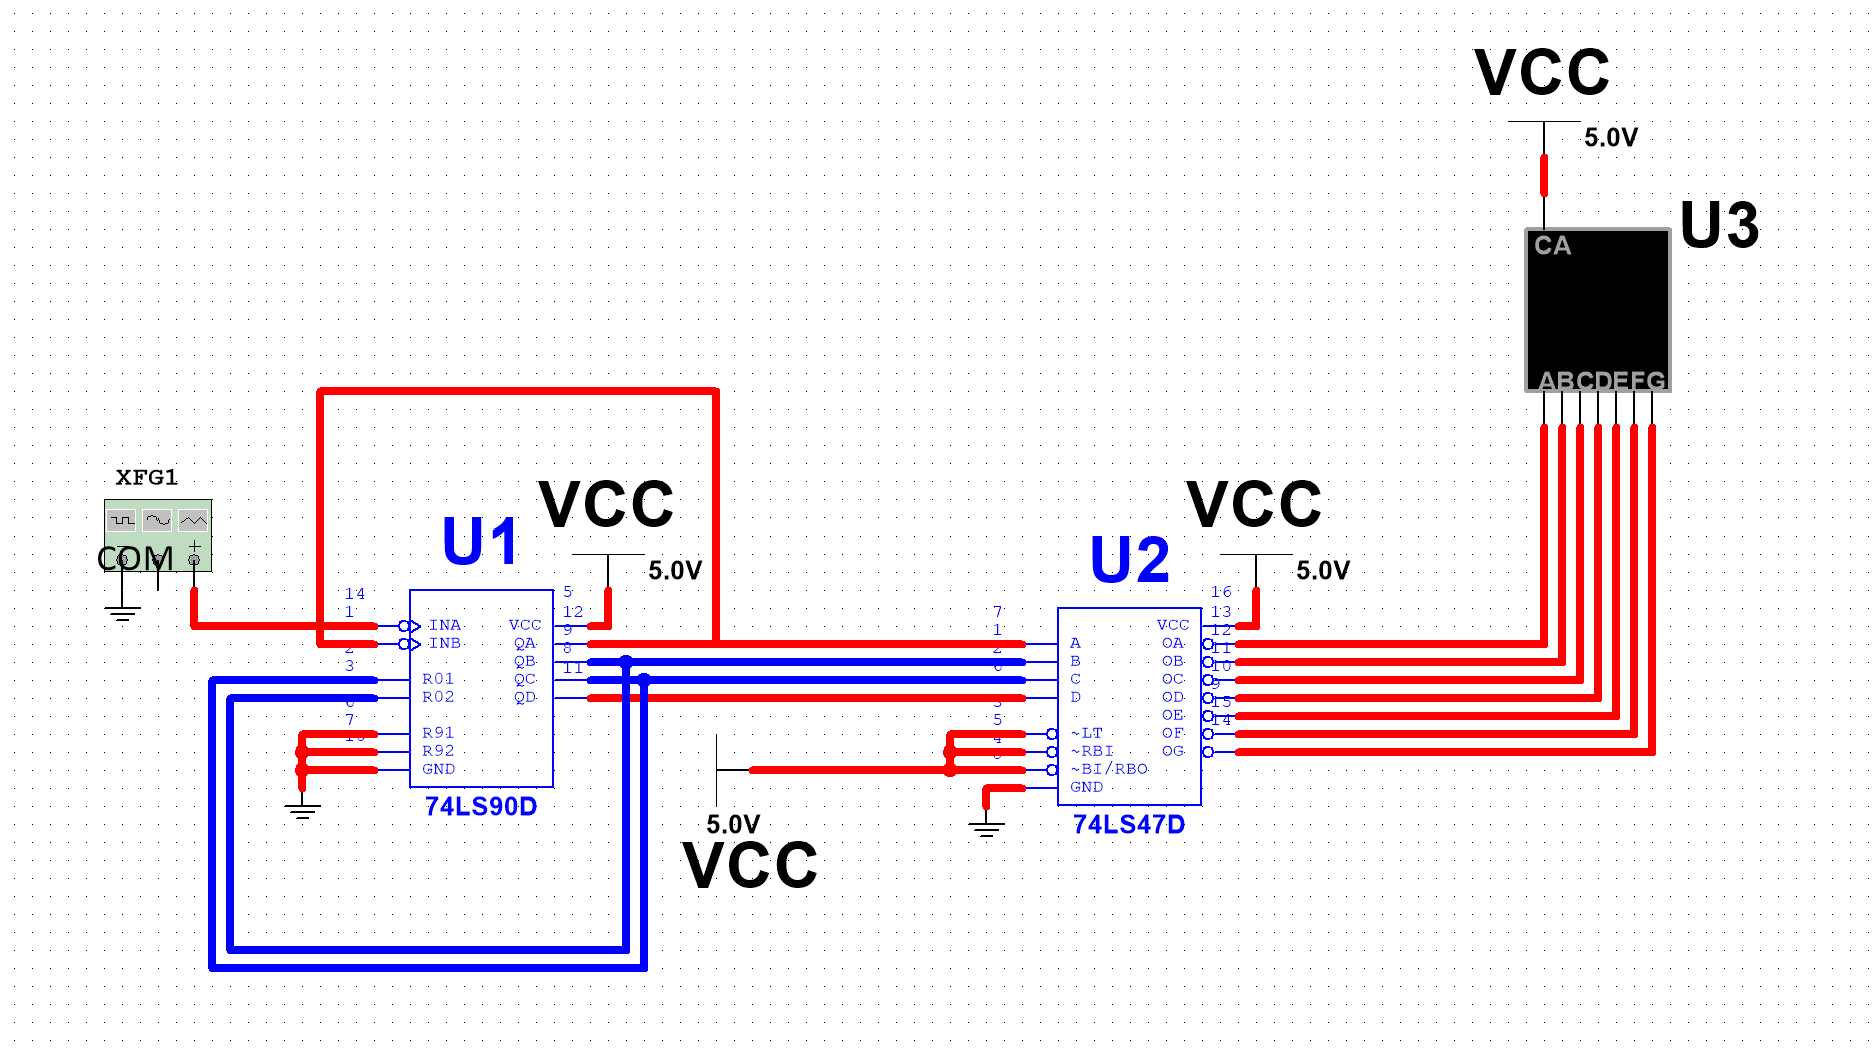
\includegraphics[width=0.8\textwidth]{design/6-0 circuit.png}
    \end{center}
    \caption{六进制计数器(置零法):原理电路}
    \label{6-0 theory cir}
\end{figure}

\subsubsection{电路实验}
\par 依据原理图,搭建硬件电路如图\ref{6 cir}所示。输入信号INA接信号发生器方波。方波参数为高电平\SI{5}{\volt},低电平\SI{0}{\volt},频率\SI{2}{\hertz}。

\begin{figure}[H]
    \begin{center}
        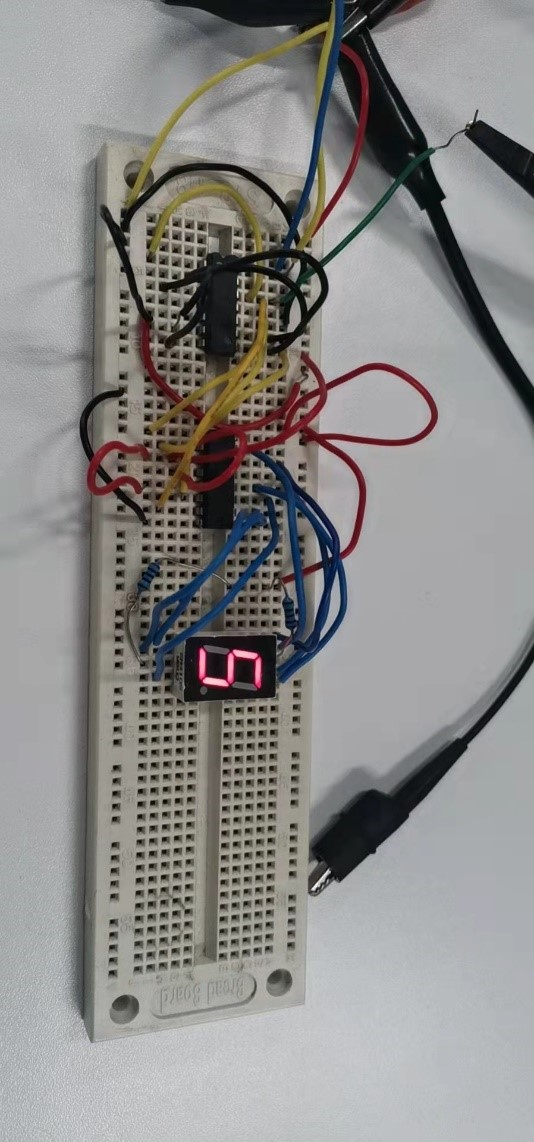
\includegraphics[width=0.8\textwidth]{6-0/circuit.jpg}
    \end{center}
    \caption{六进制计数器(置零法):硬件电路}
    \label{6 cir}
\end{figure}

\par 打开电源、打开信号源,观察实验现象。\SI{3}{\hertz}时电路现象已录制为"六进制计数器(置零法).mp4",附在邮件插件中。
\par 加大信号源频率,使用示波器观察计数器各引脚输出。其中信道1为时钟信号,信道2分别为各位输出。实验结果如图\ref{6-0 osci}所示。

\begin{figure}[H]
    \centering
    \subfigure[QA]{
    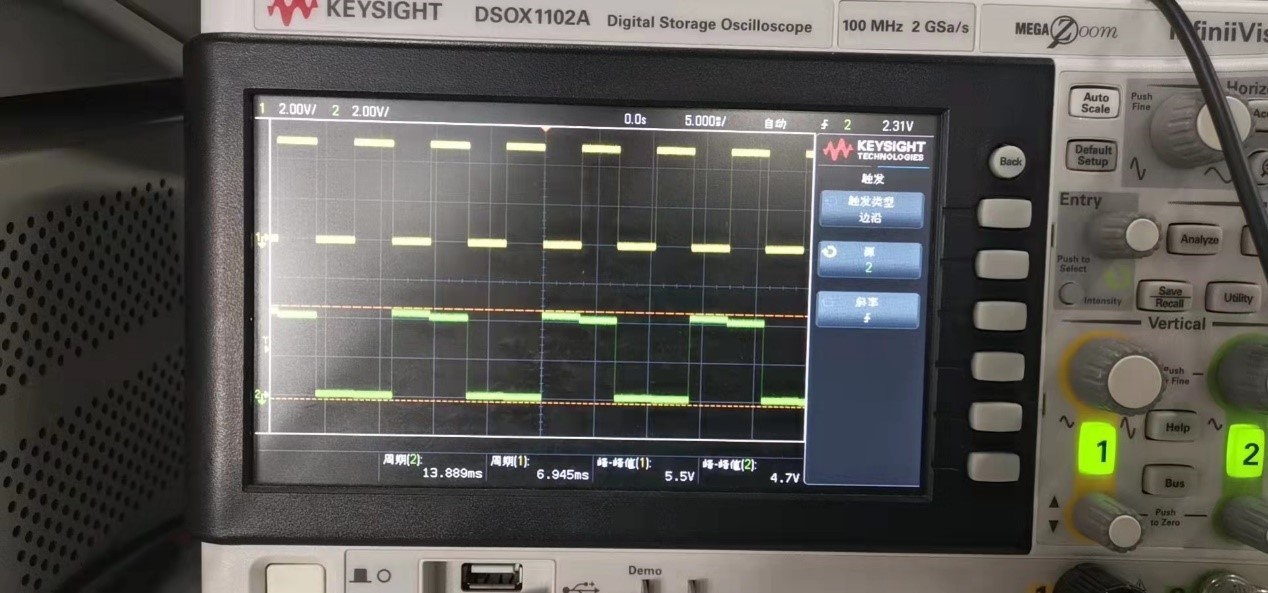
\includegraphics[width=0.45\textwidth]{6-0/QA.jpg}}
    \subfigure[QB]{
    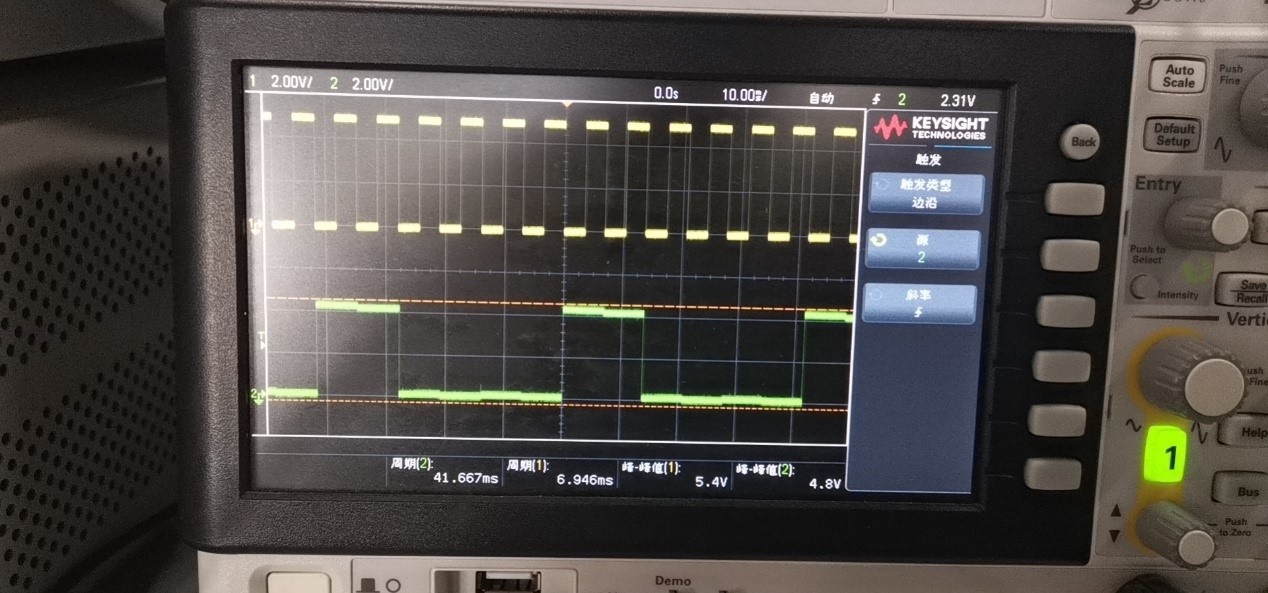
\includegraphics[width=0.45\textwidth]{6-0/QB.jpg}}
    \subfigure[QC]{
    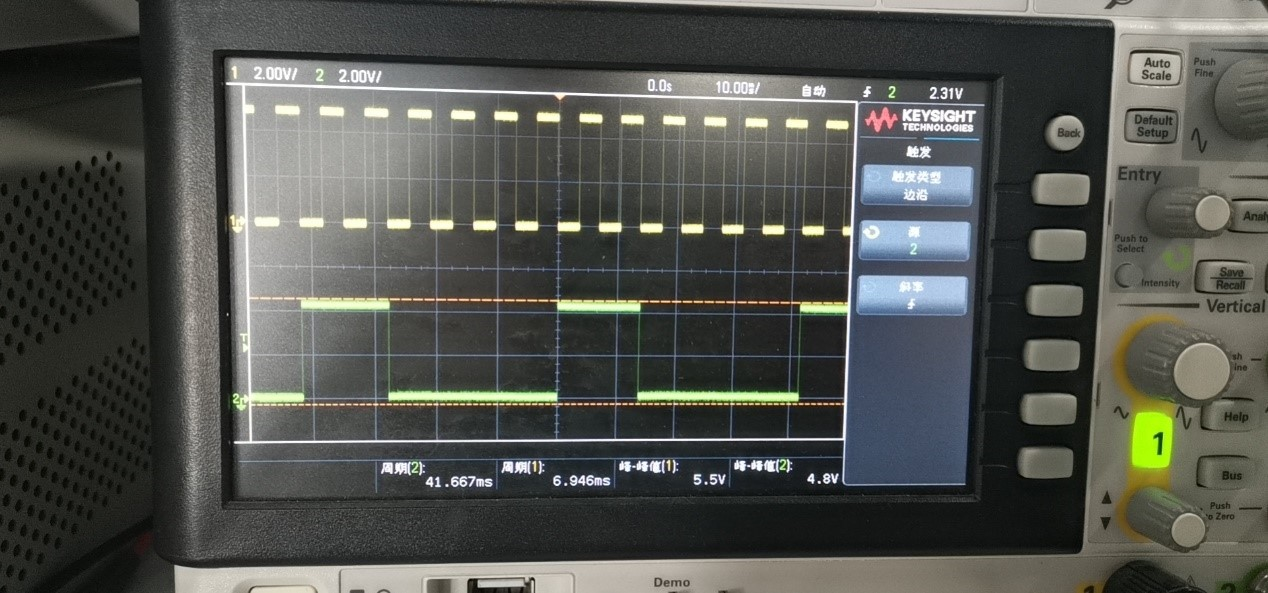
\includegraphics[width=0.45\textwidth]{6-0/QC.jpg}}
    \subfigure[QD]{
    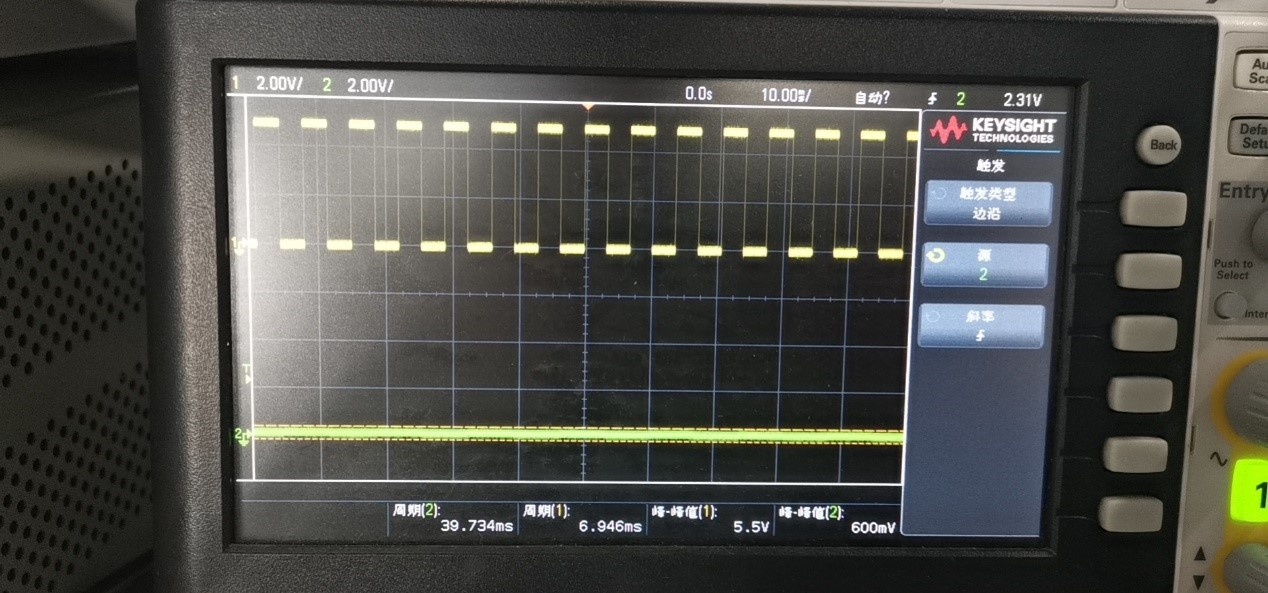
\includegraphics[width=0.45\textwidth]{6-0/QD.jpg}}
    \caption{六进制计数器(置零法):引脚波形}
    \label{6-0 osci}
\end{figure}

\par 可以看到,电路现象与各引脚波形与理论相符,成功搭建了置零法实现的六进制计数器硬件电路。

\subsection{六进制计数器:置九法}
\subsubsection{原理电路}
\par 实验电路原理图如\ref{6-9 theory cir}所示。在十进制计数器的基础上,将QA、QC引回电路置九端,使得电路输出二进制5,即“0101”时,计数器跳变到状态9。由此使计数器输出在0、1、2、3、4、9,共计6个稳态间跳变,实现六进制计数器。

\begin{figure}[H]
    \begin{center}
        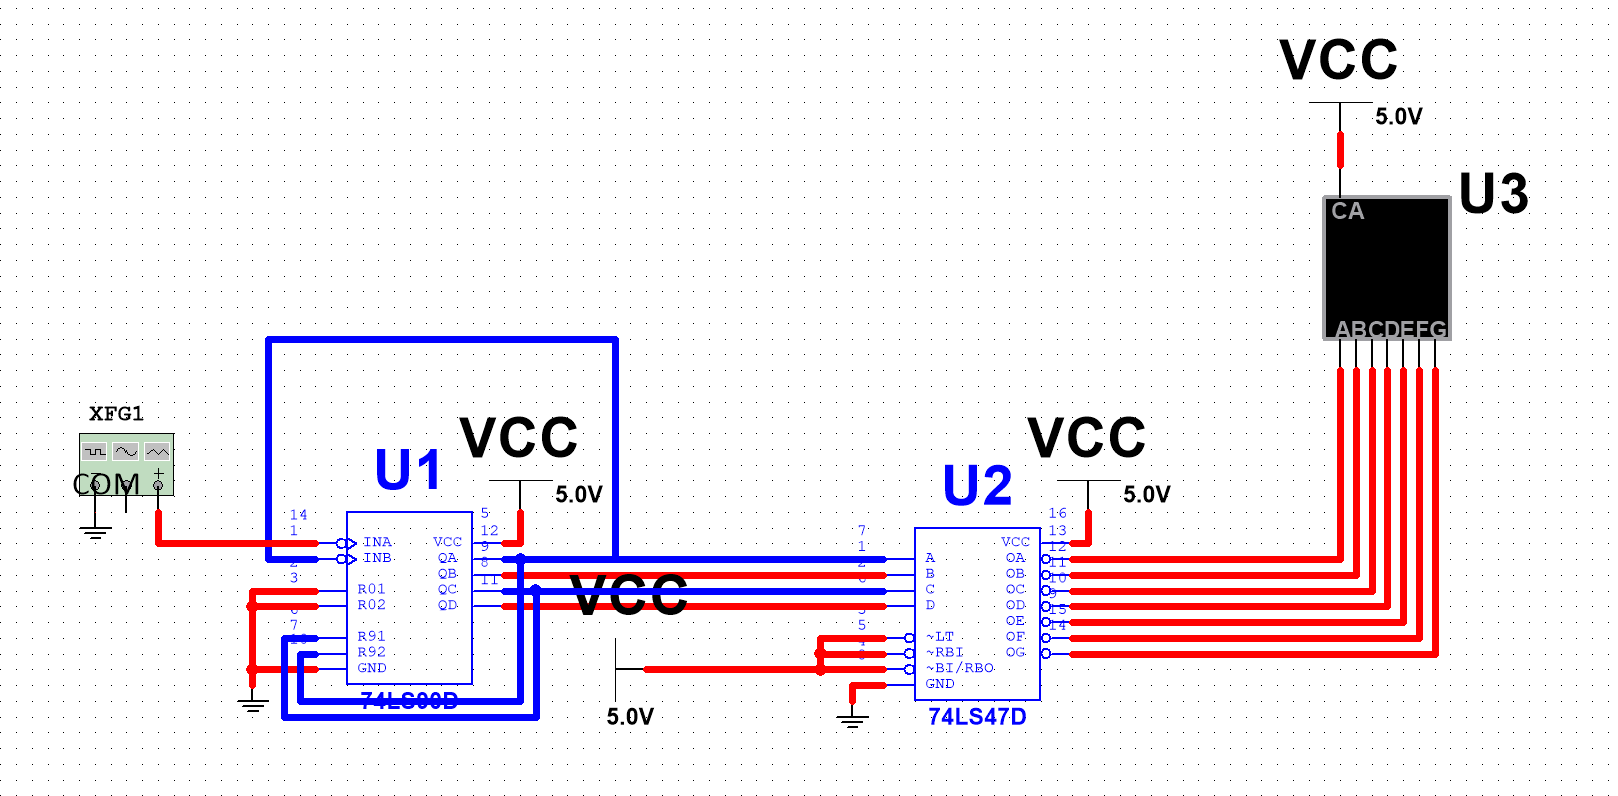
\includegraphics[width=0.8\textwidth]{design/6-9 circuit.png}
    \end{center}
    \caption{六进制计数器(置九法):原理电路}
    \label{6-9 theory cir}
\end{figure}

\subsubsection{电路实验}
\par 依据原理图,搭建硬件电路如图\ref{6-9 cir}所示。输入信号INA接信号发生器方波。方波参数为高电平\SI{5}{\volt},低电平\SI{0}{\volt},频率\SI{2}{\hertz}。

\begin{figure}[H]
    \begin{center}
        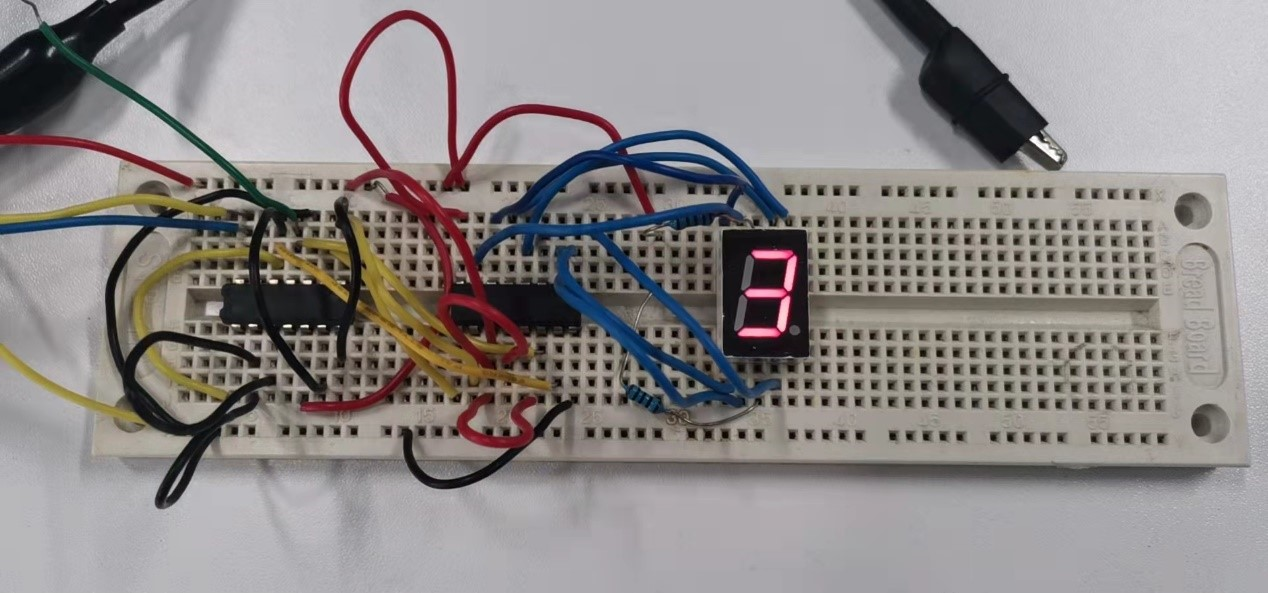
\includegraphics[width=0.8\textwidth]{6-9/circuit.jpg}
    \end{center}
    \caption{六进制计数器(置九法):硬件电路}
    \label{6-9 cir}
\end{figure}

\par 打开电源、打开信号源,观察实验现象。\SI{3}{\hertz}时电路现象已录制为"六进制计数器(置九法).mp4",附在邮件插件中。
\par 加大信号源频率,使用示波器观察计数器各引脚输出。其中信道1为时钟信号,信道2分别为各位输出。实验结果如图\ref{6-9 osci}所示。

\begin{figure}[H]
    \centering
    \subfigure[QA]{
    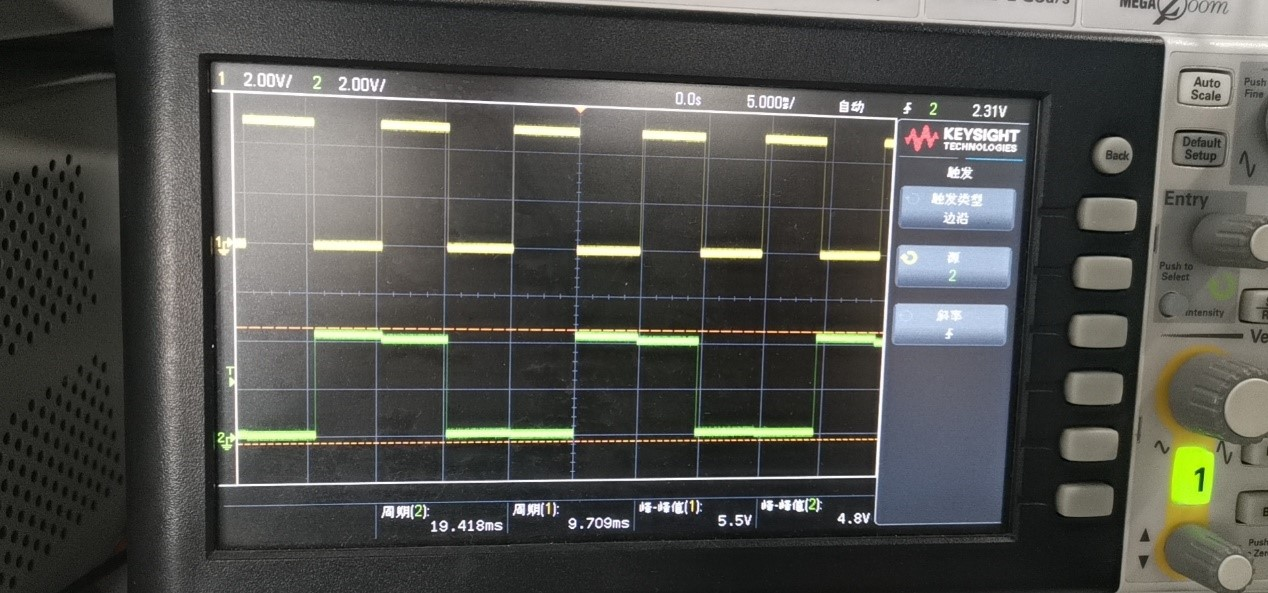
\includegraphics[width=0.45\textwidth]{6-9/QA.jpg}}
    \subfigure[QB]{
    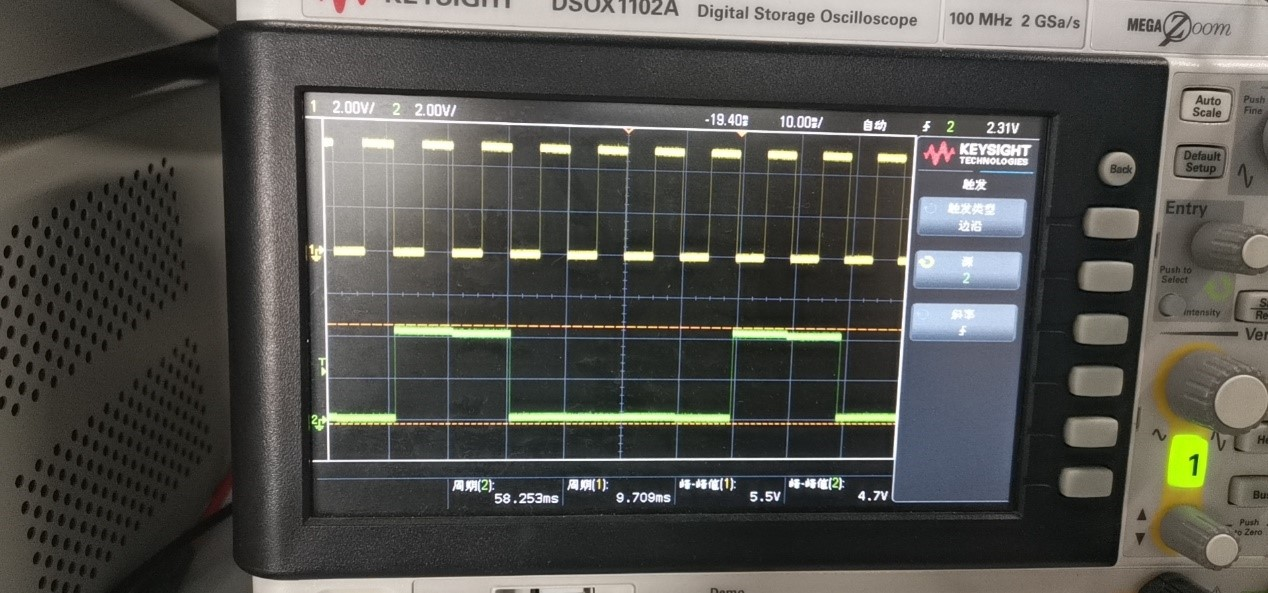
\includegraphics[width=0.45\textwidth]{6-9/QB.jpg}}
    \subfigure[QC]{
    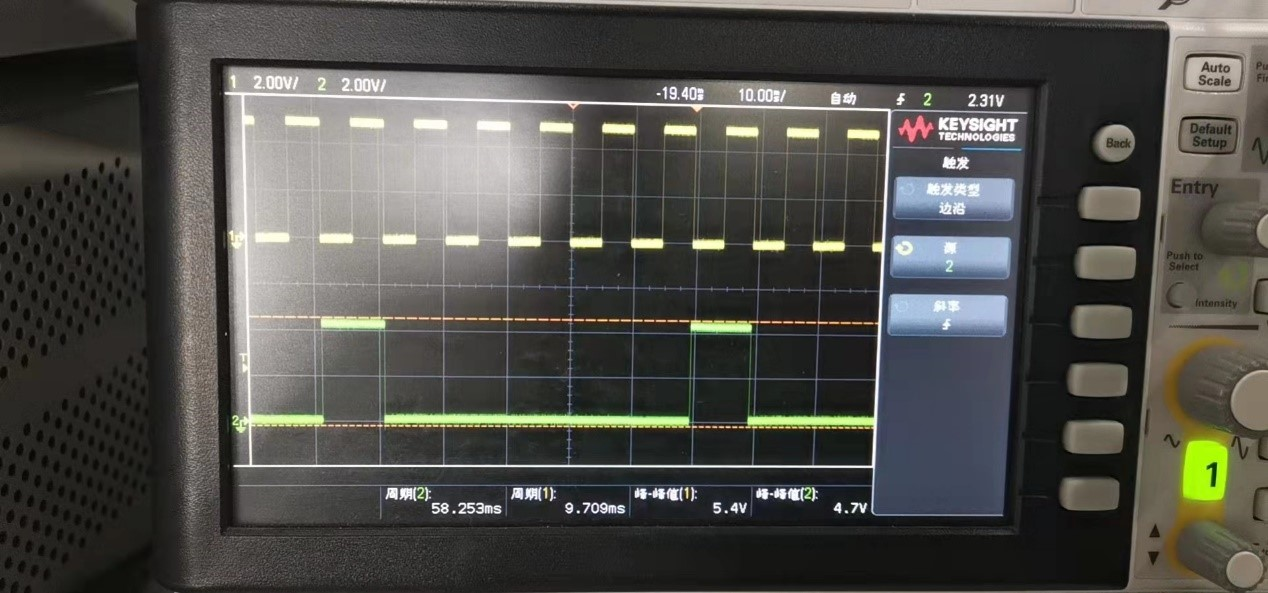
\includegraphics[width=0.45\textwidth]{6-9/QC.jpg}}
    \subfigure[QD]{
    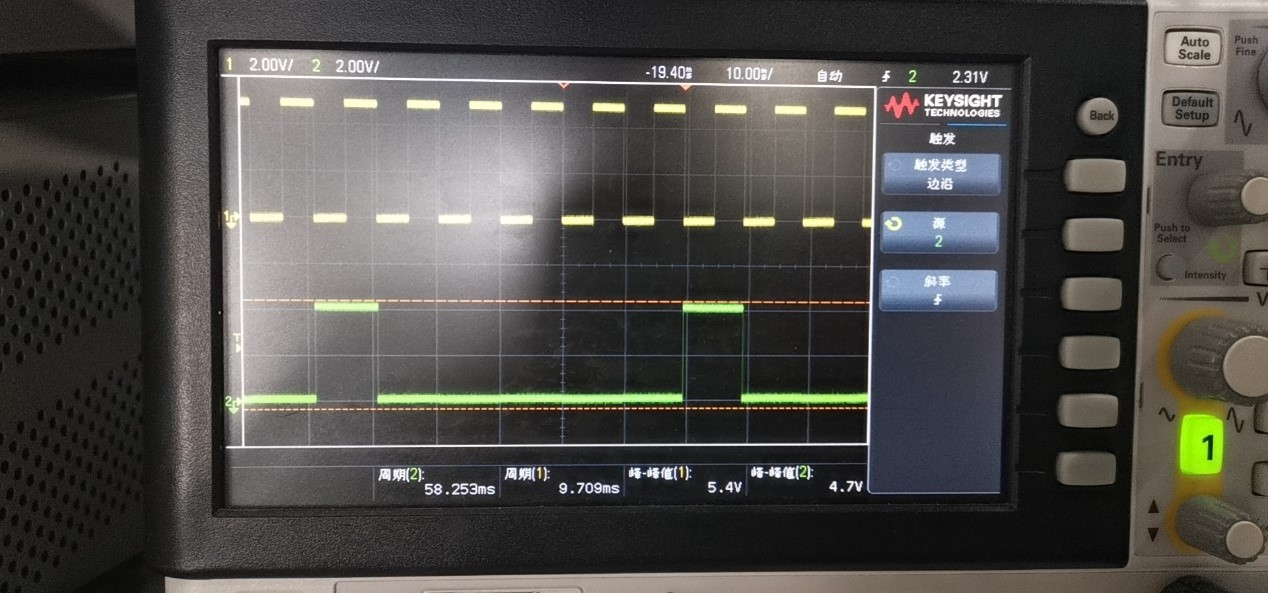
\includegraphics[width=0.45\textwidth]{6-9/QD.jpg}}
    \caption{六进制计数器(置九法):引脚波形}
    \label{6-9 osci}
\end{figure}

\par 可以看到,电路现象与各引脚波形与理论相符,成功搭建了置九法实现的六进制计数器硬件电路。


\subsection{24进制计数器}
\subsubsection{原理电路}
\par 首先,使用两位十进制计数器连接成为异步进位的100进制计数器。其中高位10进制计数器的时钟信号使用低位10进制计数器的QD引脚波形。使得低位当且仅当由9变0时,产生下降沿,使得高位计数器计数值加一。100进制计数器原理如如图
\ref{100 theory cir}所示。

\begin{figure}[H]
    \begin{center}
        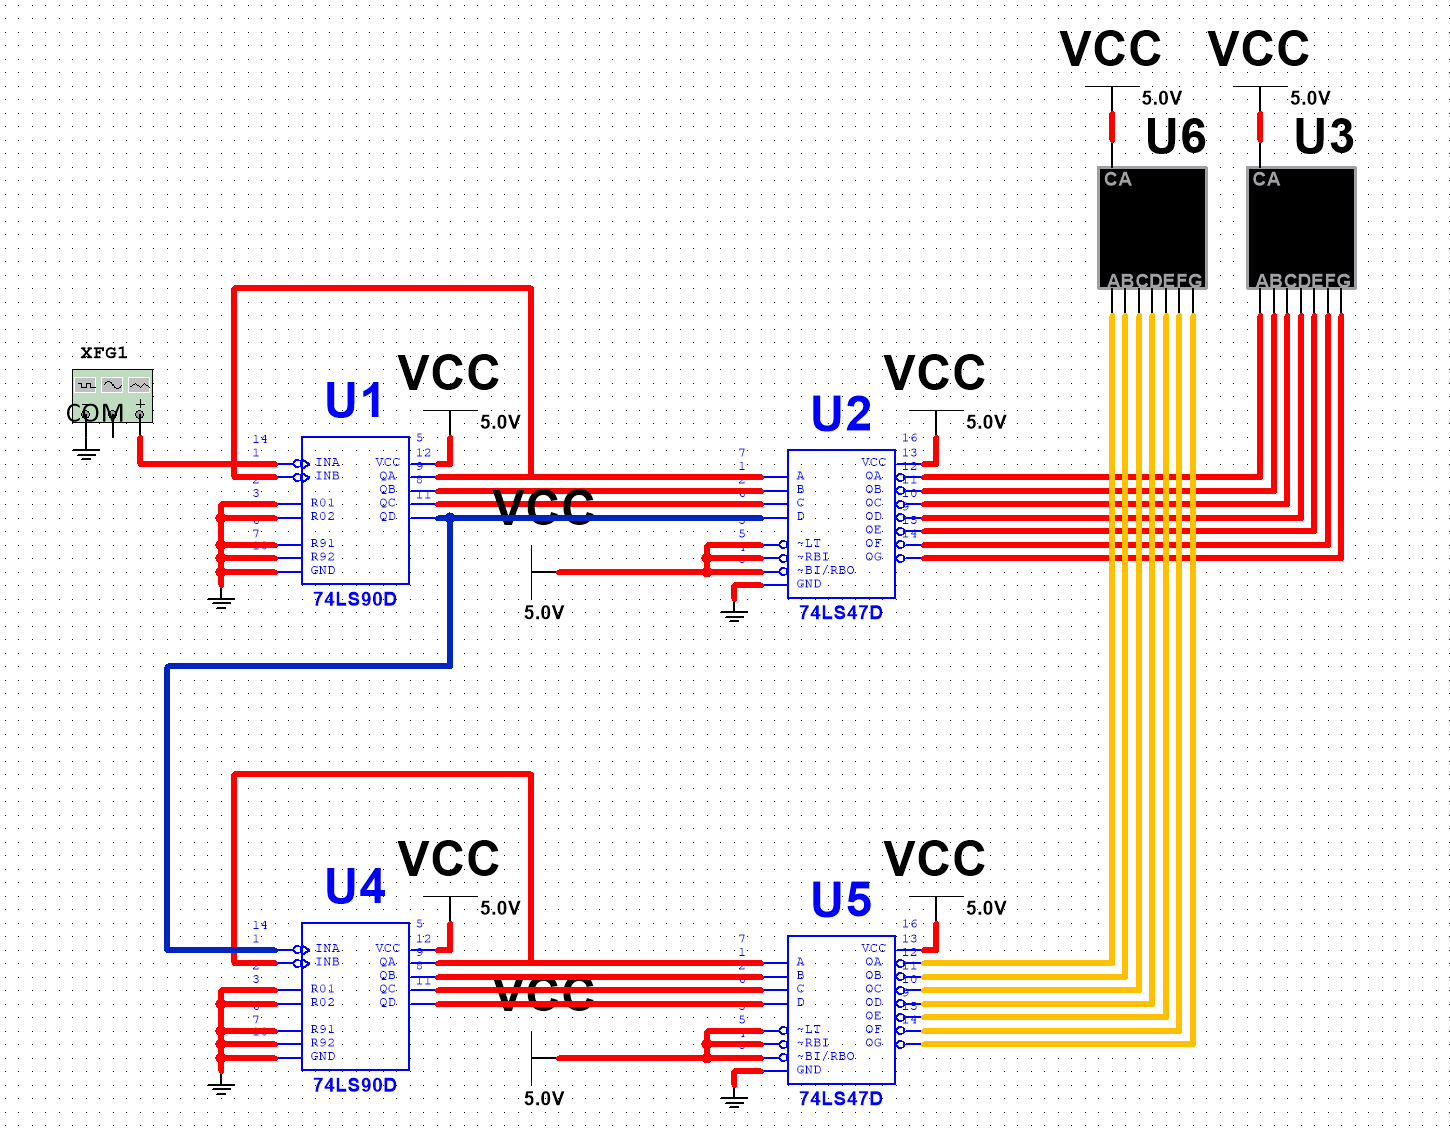
\includegraphics[width=0.8\textwidth]{design/100 circuit.png}
    \end{center}
    \caption{100进制计数器:原理电路}
    \label{100 theory cir}
\end{figure}

在此基础上,将高位的QB、低位的QC分别引到两位计数器的置零端上。由于不能够使用额外的门电路,此处使用的方式为部分译码,当电路从0计数递增至24时,置零条件第一次全部满足,使得电路在计数23后跳回00,构成24进制计数器。24进制计数器的原理电路如图\ref{24 theory cir}所示。

\begin{figure}[H]
    \begin{center}
        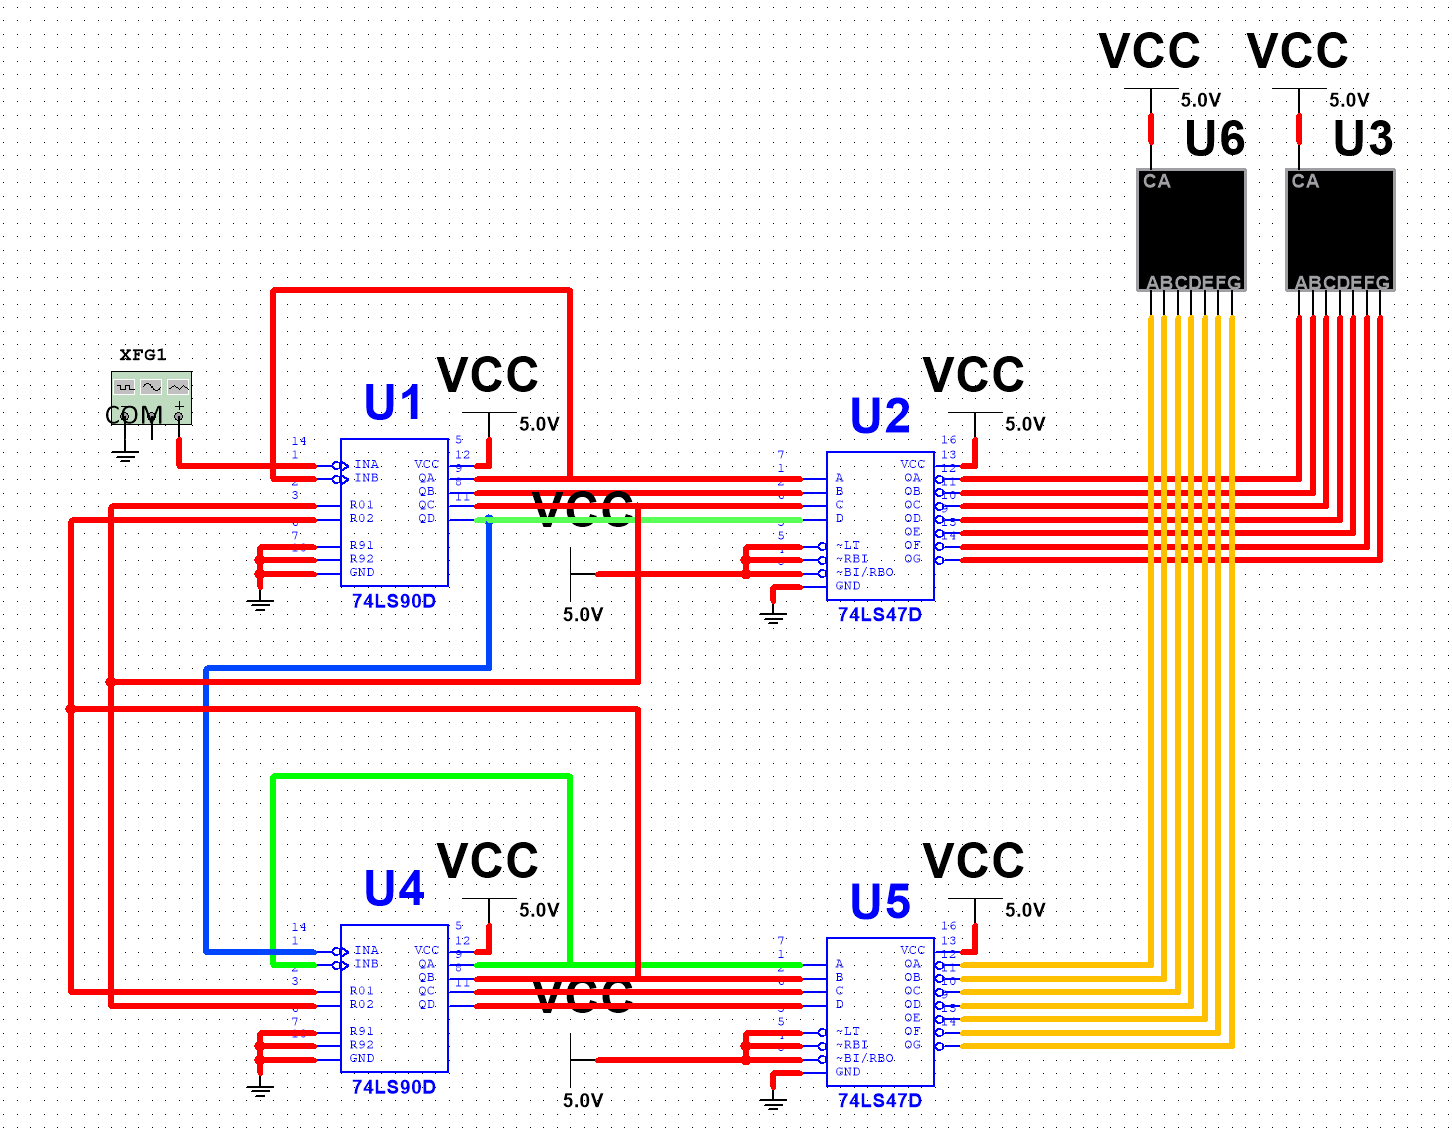
\includegraphics[width=0.8\textwidth]{design/24 circuit.png}
    \end{center}
    \caption{24进制计数器:原理电路}
    \label{24 theory cir}
\end{figure}

\subsubsection{电路实验}
\par 依据原理图,搭建硬件电路如图\ref{24 cir}所示,其中下侧的面包板上为计数器高位部分。输入信号INA接信号发生器方波。方波参数为高电平\SI{5}{\volt},低电平\SI{0}{\volt},频率\SI{2}{\hertz}。

\begin{figure}[H]
    \begin{center}
        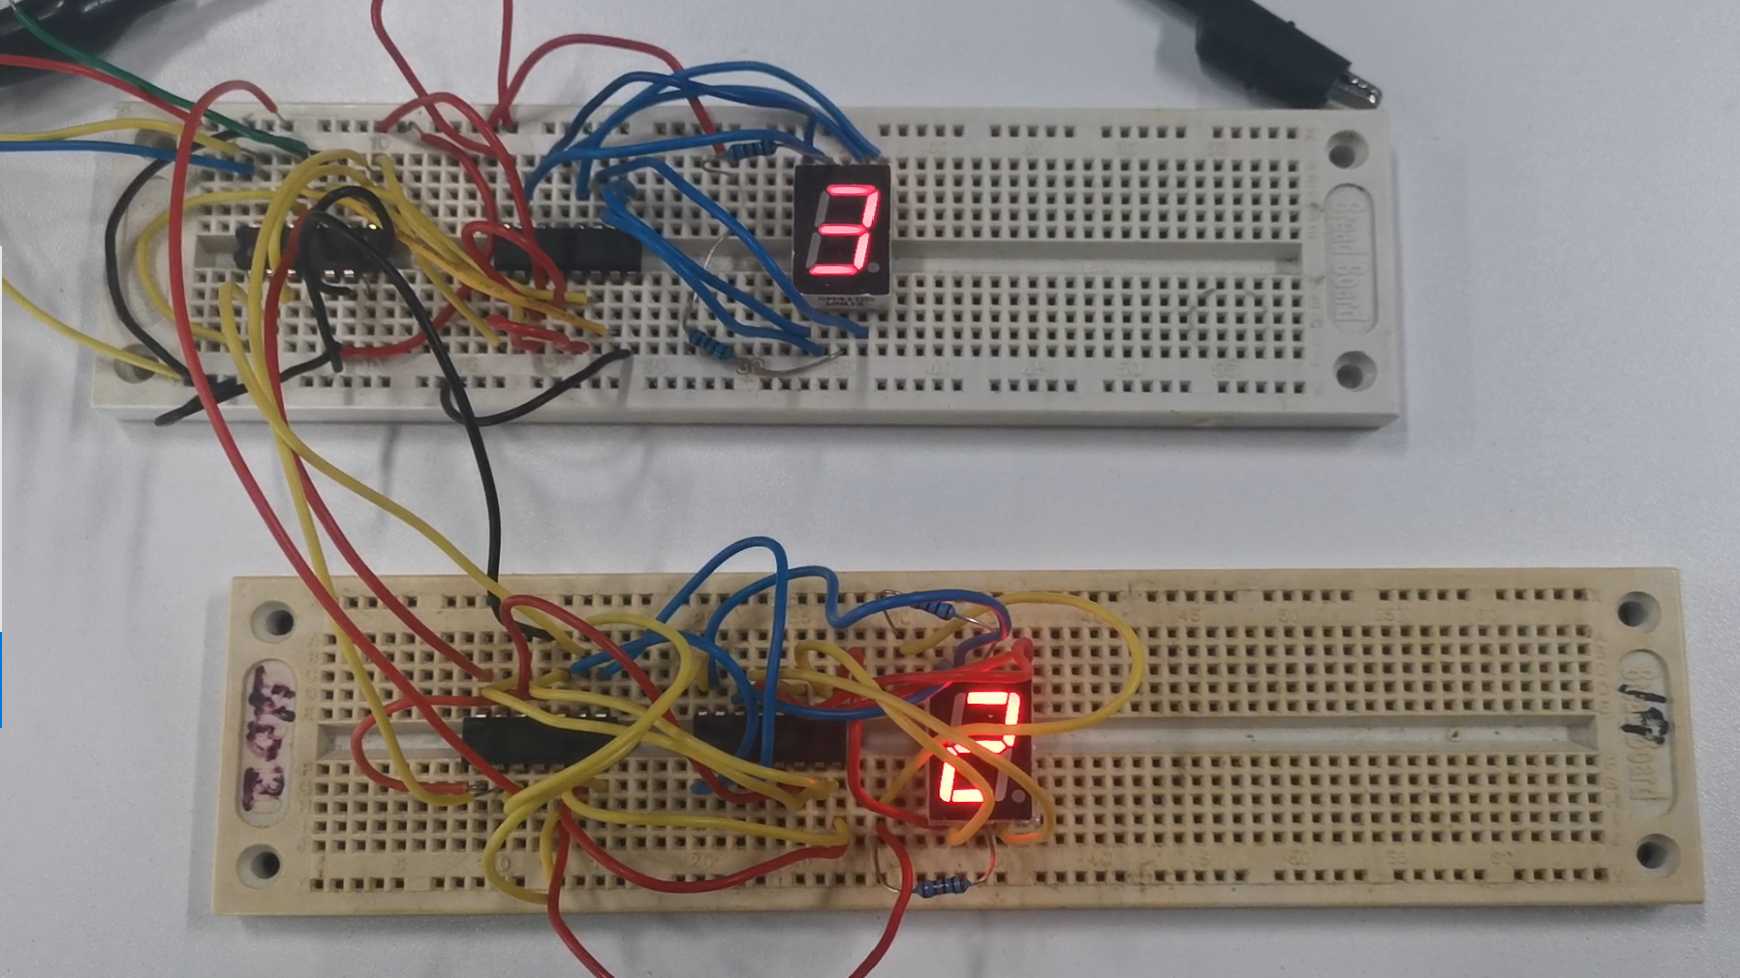
\includegraphics[width=0.8\textwidth]{24.png}
    \end{center}
    \caption{24进制计数器:硬件电路}
    \label{24 cir}
\end{figure}

\par 打开电源、打开信号源,观察实验现象。\SI{3}{\hertz}时电路现象已录制为"24进制计数器.mp4",附在邮件插件中。可以看到,电路显示状态由“00”计数递增至“23”后归零,成功构成了24进制计数器。

\subsection{38进制计数器}
\subsubsection{原理电路}
\par 首先,使用两位十进制计数器连接成为异步进位的100进制计数器。然而,若仅使用置零端搭建38进制计数器,即使使用部分译码办法,译出十位“3”时需要使用QB、QC,译出个位“8”时需要使用QD,置零端需要有3引脚才可实现。然而74LS90置零端仅有两个,故仅使用置零端无法构成38进制计数器。
\par 综合使用置九端和置零端可以实现38进制计数器。注意到虽然译出“38”需要3引脚,但若电路由于置九端跳过80~89,则在译出“98”时仅需连接高、低位QD值两计数器置零端,即可实现在电路到达状态“98”时立即置零。可以利用此性质实现38计数器,具体实现如下:
\par 在100进制计数器的基础上,将高位置九端连接高位输出的QA、QB,译出“3”的状态,使得计数器在29过后直接跳变90。
\par 将高位、低位的QD分别连接至两位的置零端上,利用部分译码使得刚才所得的电路在“98”时置零条件第一次满足,使得电路置零。
\par 由此,计数器稳态为“00”~“29”,“90”~“97”,电路在“97”后随即回到“00”,电路共计38个稳态,成功实现了38进制计数器。
\par 原理电路如图\ref{38 theory cir}

\begin{figure}[H]
    \begin{center}
        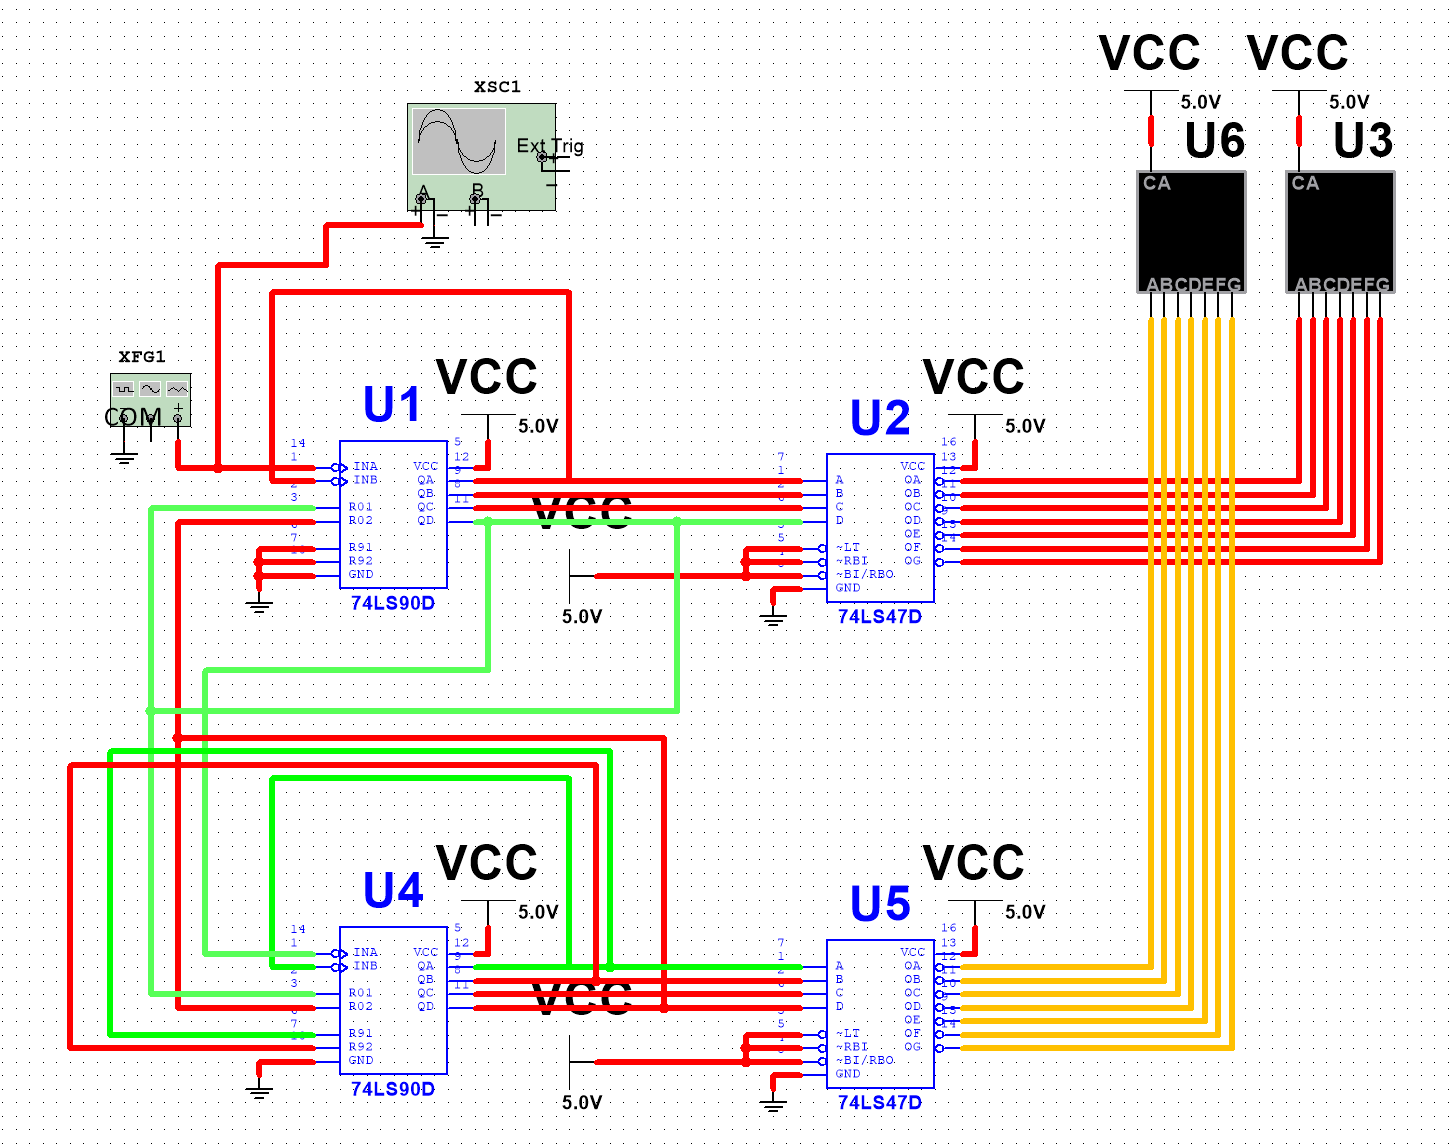
\includegraphics[width=0.8\textwidth]{design/38 circuit.png}
    \end{center}
    \caption{38进制计数器:原理电路}
    \label{38 theory cir}
\end{figure}


\subsubsection{电路实验}
\par 依据原理图,搭建硬件电路如图\ref{38 cir}所示,下侧面包板为高位电路。输入信号INA接信号发生器方波。方波参数为高电平\SI{5}{\volt},低电平\SI{0}{\volt},频率\SI{2}{\hertz}。

\begin{figure}[H]
    \begin{center}
        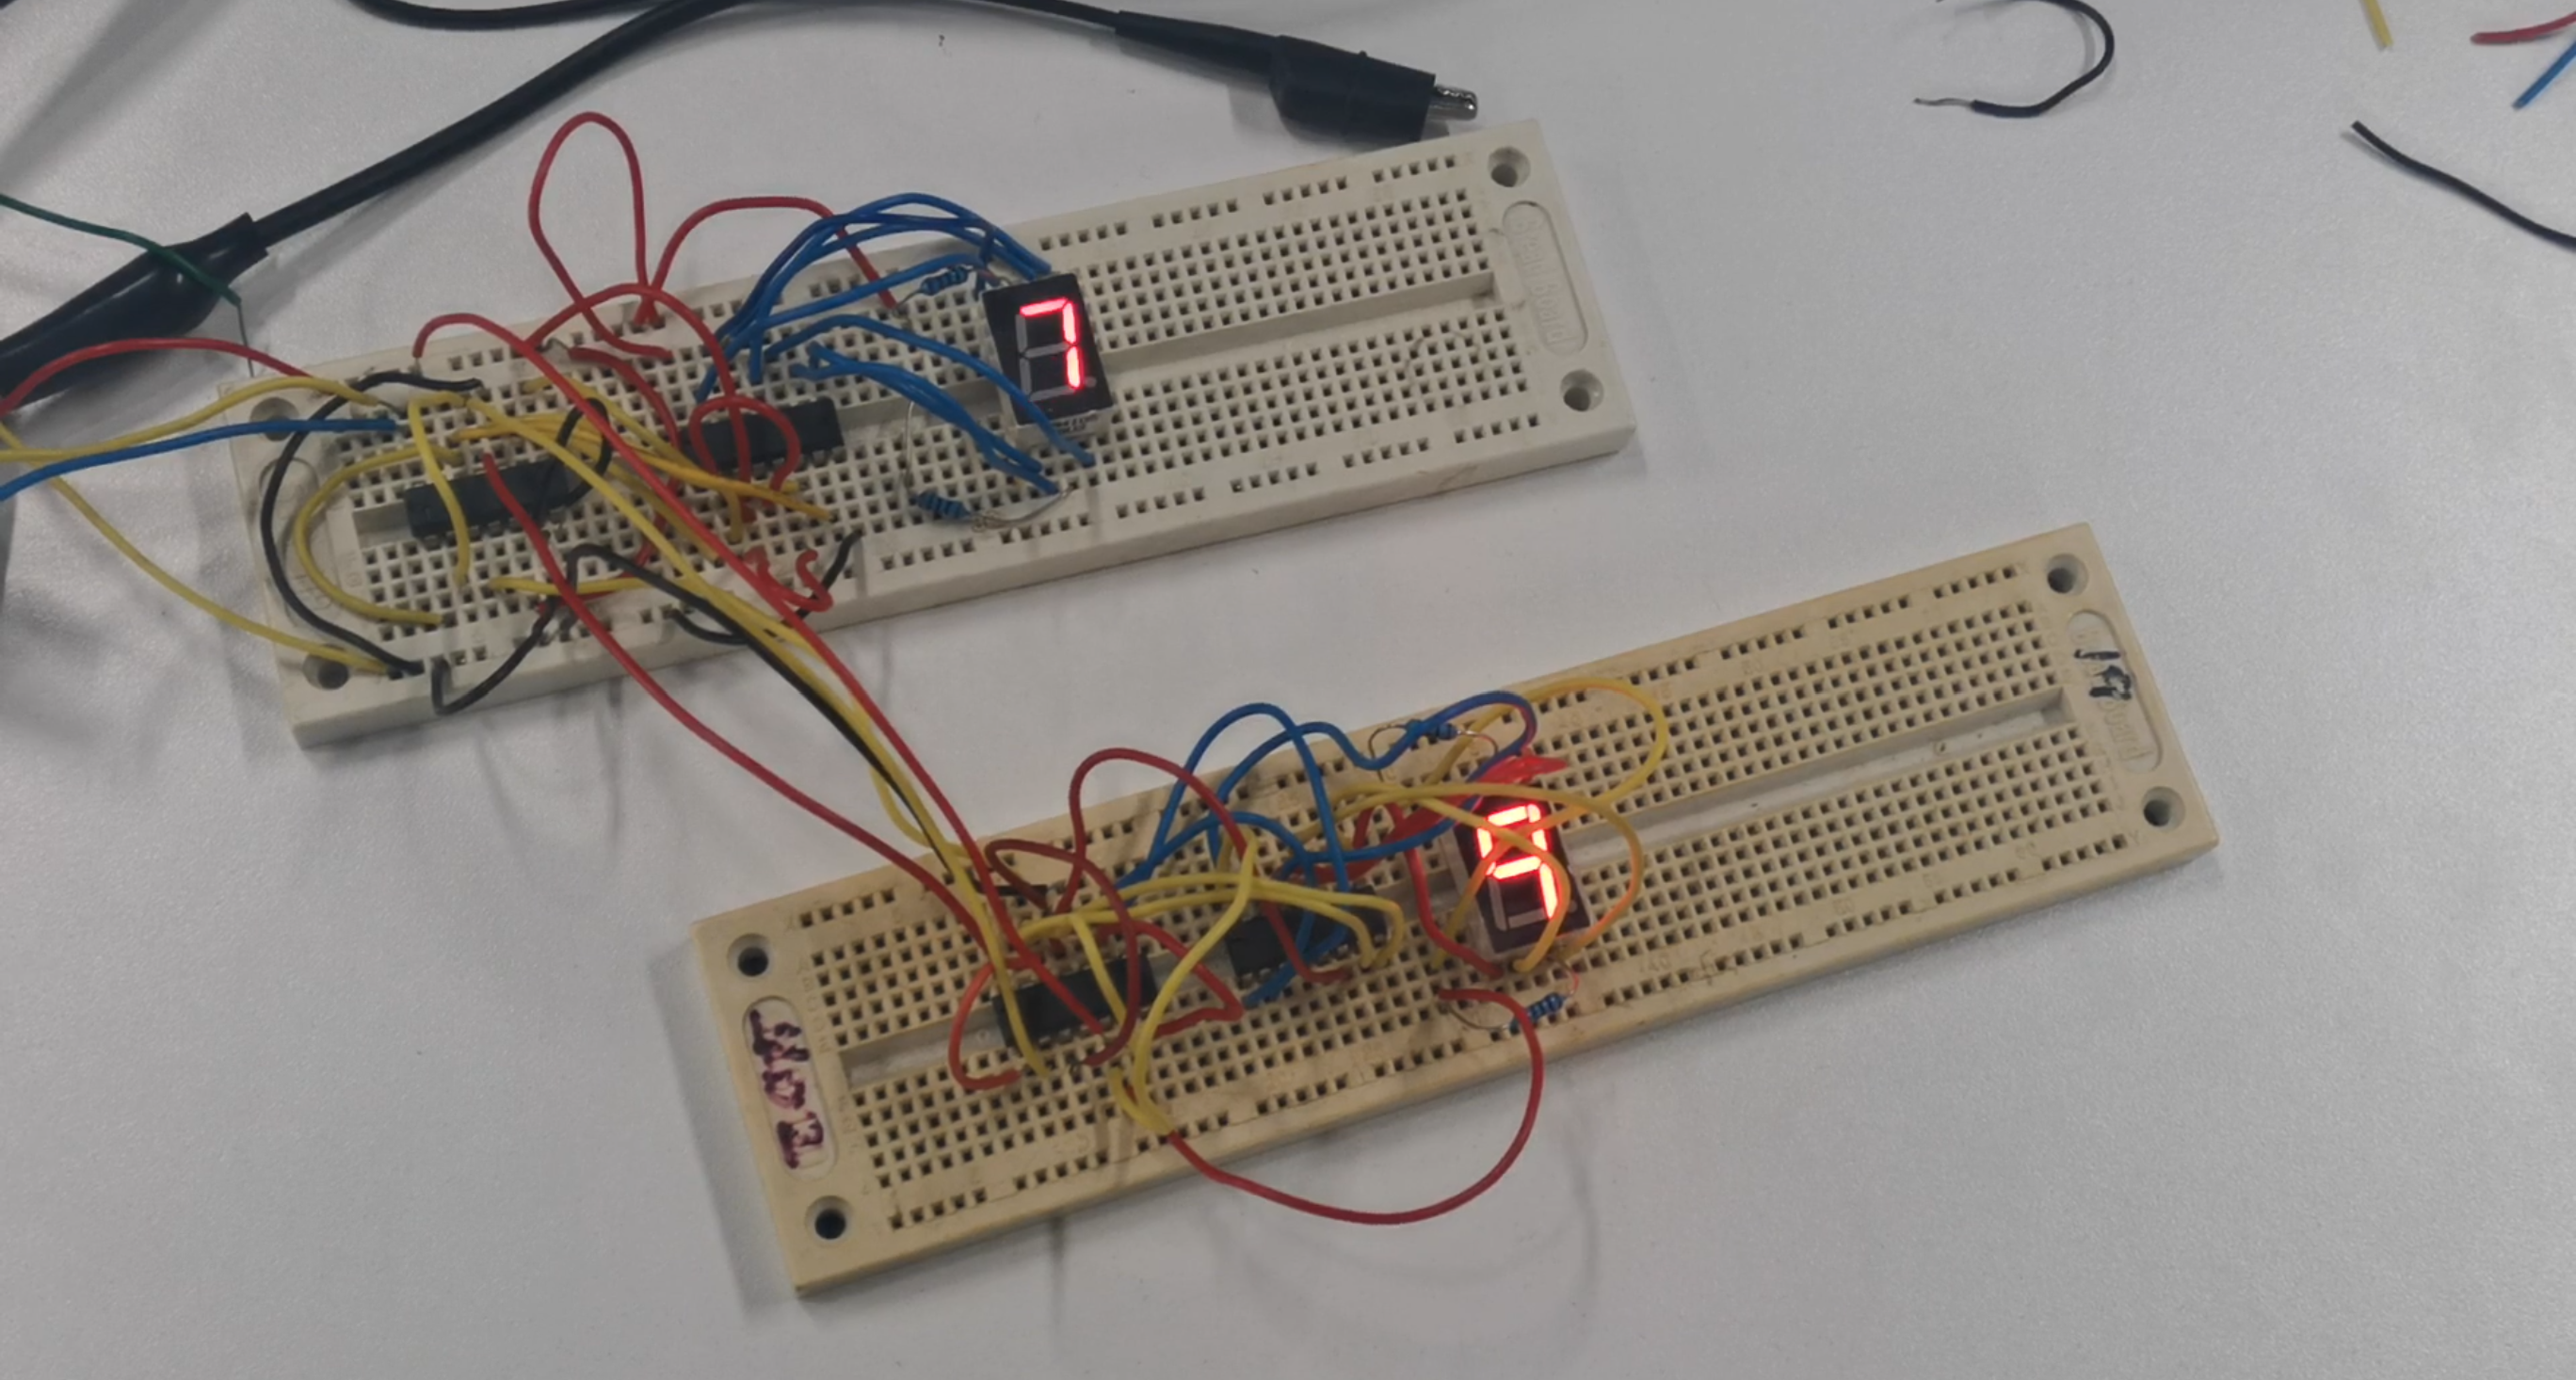
\includegraphics[width=0.8\textwidth]{38.png}
    \end{center}
    \caption{38进制计数器:硬件电路}
    \label{38 cir}
\end{figure}

\par 打开电源、打开信号源,观察实验现象。\SI{3}{\hertz}时电路现象已录制为"38进制计数器.mp4",附在邮件插件中。可以看到,电路显示状态由“00”计数递增至“29”后跳变至“90”,继续递增至“97”后归零,成功构成了38进制计数器。

\subsubsection{讨论}
实验过程中帮助其他同学解决了一些问题,在此讨论如下:
\paragraph{不能使用置九法实现九进制计数器} 有其他小组同学希望构建九进制计数器,利用\(38 = 9 \times 4 + 2\),译出42,实现38进制计数器。从译码的角度这确实是一个巧妙的实现方案,但是实现中遇到了问题。由于在42时需要置零,占用置零端,9进制计数器只能通过置九法实现。然而,74LS90两置九端都是高电平有效,为了使计数器在8,即二进制“1000”时跳变至9,不使用门电路的条件下只能将QD同时连接两置九端。然而这样操作会使电路在状态“9”,即二进制输出“1001”时电路置九端仍然有效,使得电路卡死在输出“9”的状态,无法实现38进制的功能。
\paragraph{构成两位计数器的时候需要使用相同的电源} 在构成24进制计数器以及38进制计数器时,需要连接相同的电源进行供电。这是由于电源的零电位参考点(地位)可能不相同,使得电路电位混乱,产生不可预见的电路表现。实验中遇到的情况为电路高位在0、1、4、5、0、1这几个状态中不断循环。


\section{实验总结}

成功使用74LS90、74LS47以及数码管成功实现了十进制计数器、置零法以及置九法实现的六进制计数器、24进制计数器、38进制计数器。熟悉了使用硬件构建数字电路的操作,

\section*{原始数据}
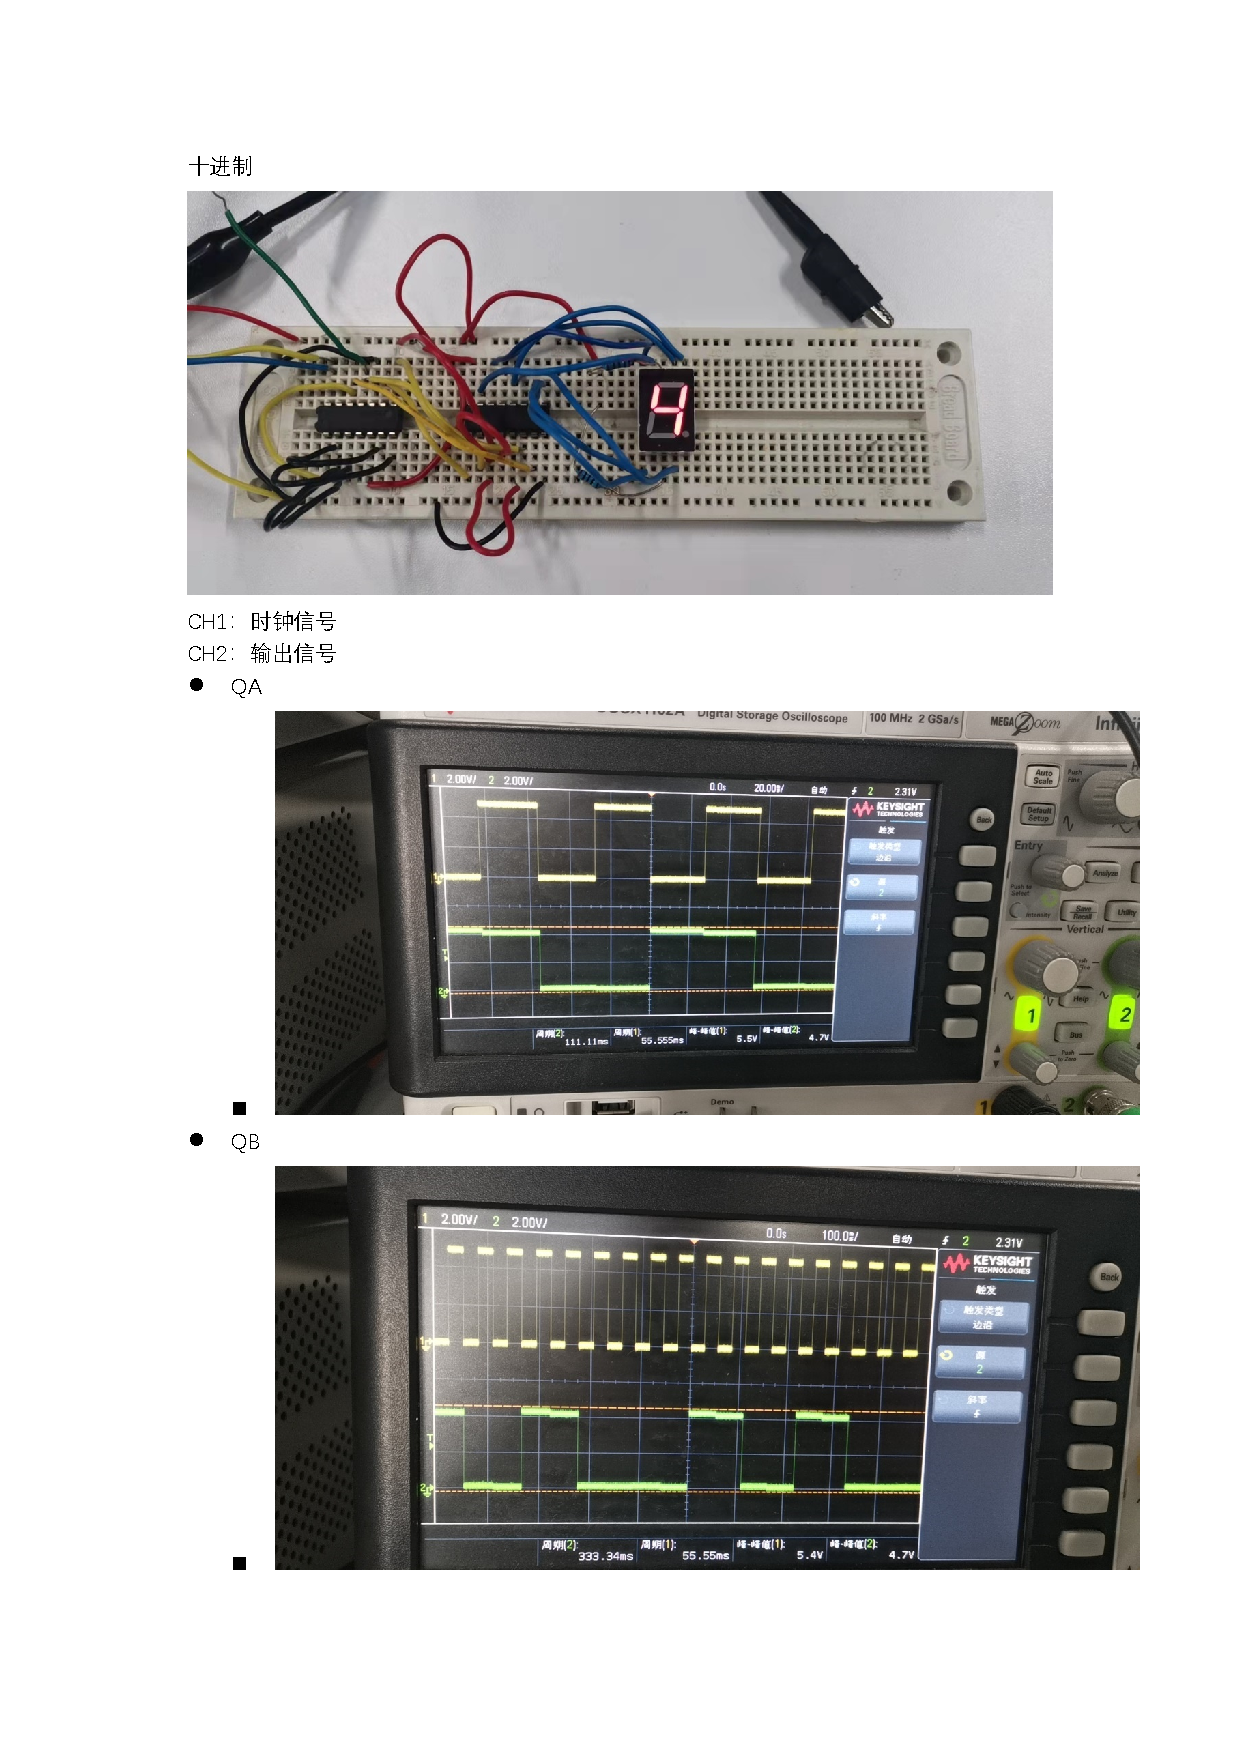
\includepdf[pages=1-6]{data.pdf}

\begin{figure}[H]
    \begin{center}
        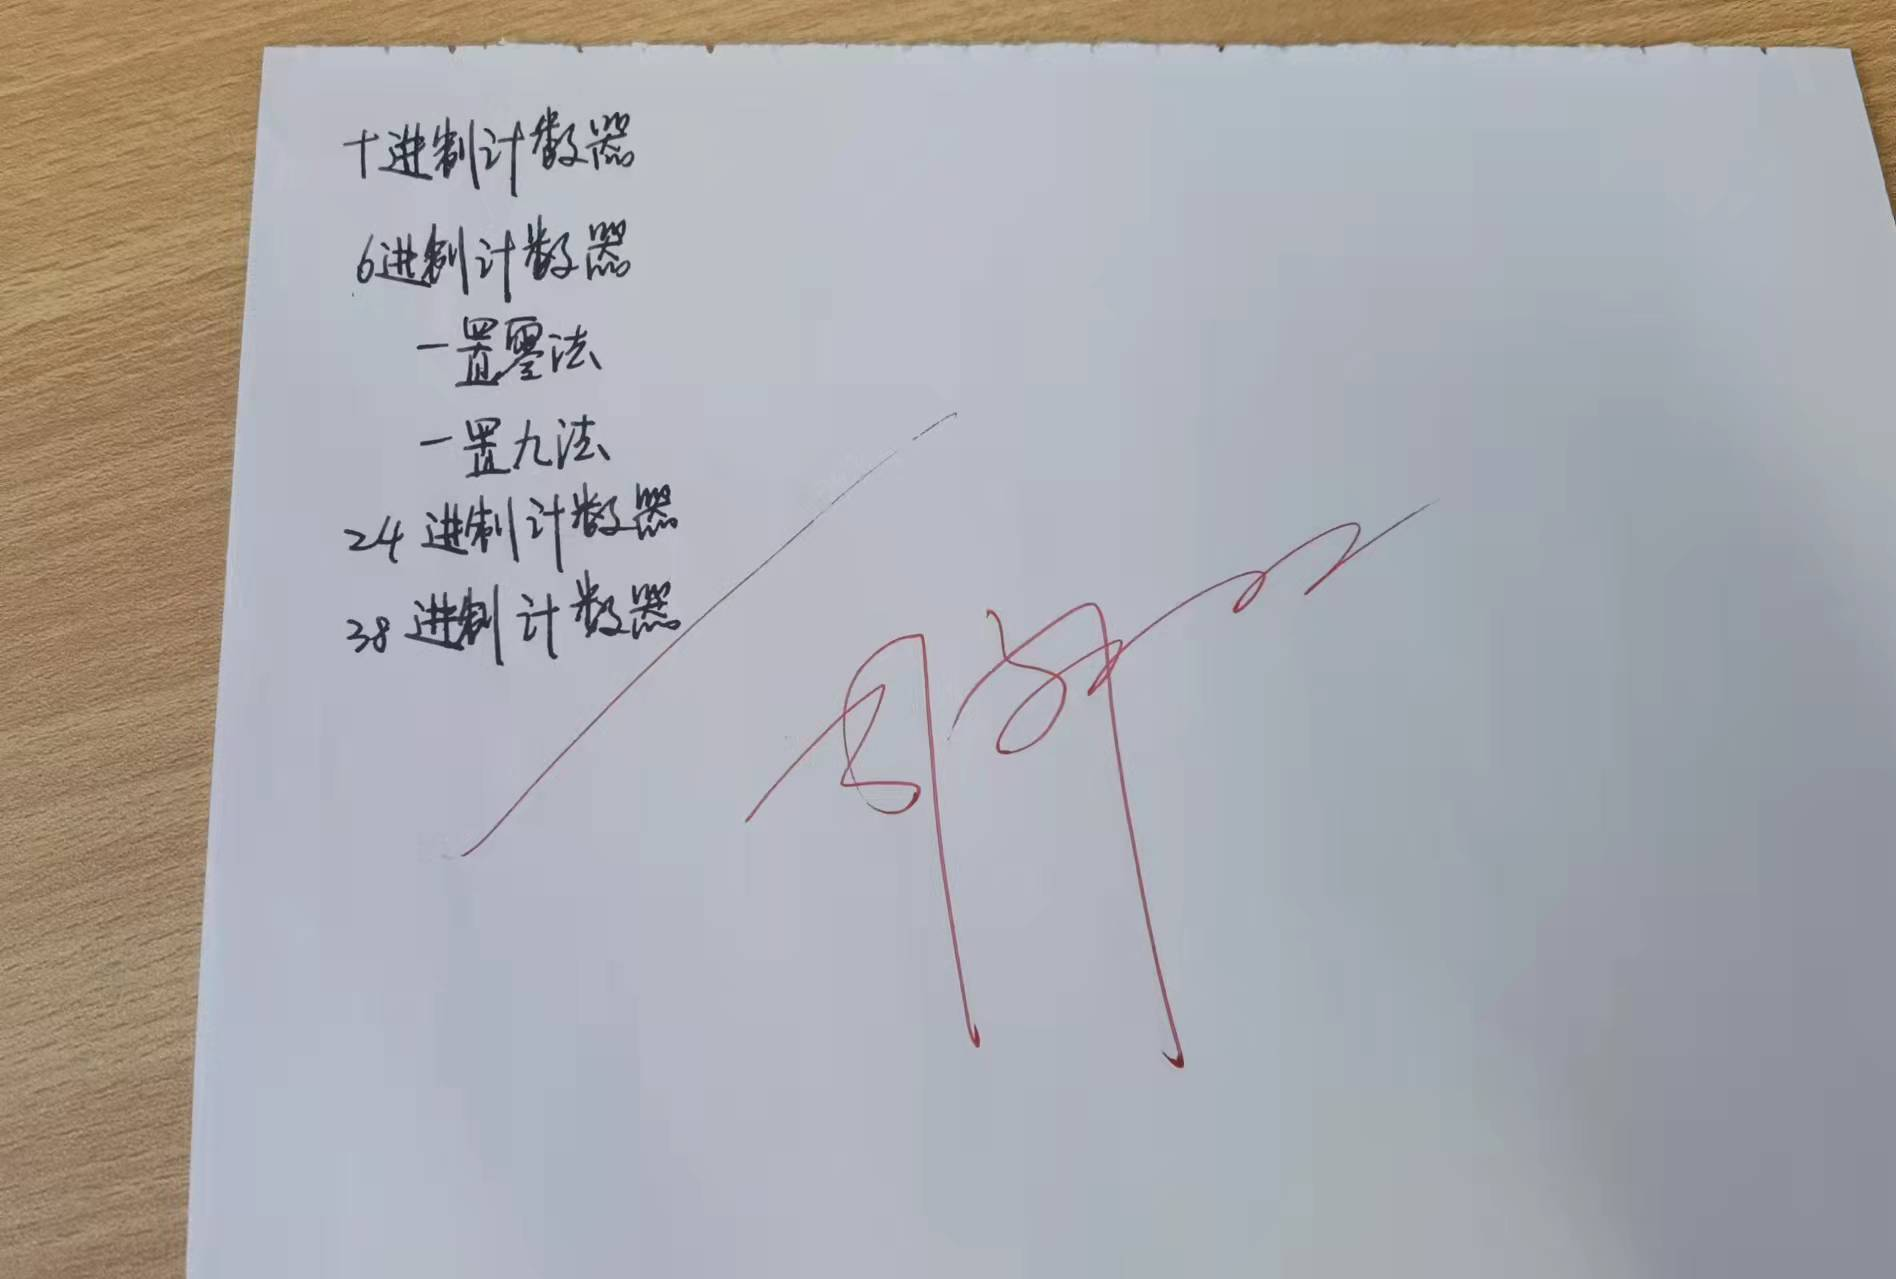
\includegraphics[width=0.8\textwidth]{sign.jpg}
    \end{center}
\end{figure}

\end{document}